% mn2esample.tex
%
% v2.1 released 22nd May 2002 (G. Hutton)
%
% The mnsample.tex file has been amended to highlight
% the proper use of LaTeX2e code with the class file
% and using natbib cross-referencing. These changes
% do not reflect the original paper by A. V. Raveendran.
%
% Previous versions of this sample document were
% compatible with the LaTeX 2.09 style file mn.sty
% v1.2 released 5th September 1994 (M. Reed)
% v1.1 released 18th July 1994
% v1.0 released 28th January 1994

\documentclass[useAMS,usenatbib,times,letter,amssymb]{mn2e}
\usepackage{graphicx, float, amsmath,epsfig,times,amssymb,color,verbatim}
% If your system does not have the AMS fonts version 2.0 installed, then
% remove the useAMS option.
%
% useAMS allows you to obtain upright Greek characters.
% e.g. \umu, \upi etc.  See the section on "Upright Greek characters" in
% this guide for further information.
%
% If you are using AMS 2.0 fonts, bold math letters/symbols are available
% at a larger range of sizes for NFSS release 1 and 2 (using \boldmath or
% preferably \bmath).
%
% The usenatbib command allows the use of Patrick Daly's natbib.sty for
% cross-referencing.
%
% If you wish to typeset the paper in Times font (if you do not have the
% PostScript Type 1 Computer Modern fonts you will need to do this to gets

% smoother fonts in a PDF file) then uncomment the next line
% \usepackage{Times}

%%%%% AUTHORS - PLACE YOUR OWN MACROS HERE %%%%%
\def\be{\begin{equation}}
\def\ee{\end{equation}}
\def\bea{\begin{eqnarray}}
\def\eea{\end{eqnarray}}
\def\ATrue{0.7}
\newcommand{\bm}[1]{\mbox{\boldmath{$#1$}}}   %this is bold italic for MNRAS
%%%%%%%%%%%%%%%%%%%%%%%%%%%%%%%%%%%%%%%%%%%%%%%%

\title[On the complementarity of galaxy clustering with cosmic shear and flux magnification.]{On the complementarity of galaxy clustering with cosmic shear and flux magnification.}
\author[C. Duncan et al.]{Christopher Duncan$^{1}$, Benjamin Joachimi$^{1}$, Alan Heavens$^{2}$, Catherine Heymans$^{1}$,\newauthor Hendrik Hildebrandt$^{3}$\\
$^{1}$Institute for Astronomy, Royal Observatory Edinburgh, Blackford Hill, Edinburgh\\
$^{2}$Imperial College London\\
$^3$}

\par
\begin{document}

\date{Submitted}

\pagerange{\pageref{firstpage}--\pageref{lastpage}} \pubyear{2012}

\maketitle

\label{firstpage}

\begin{abstract}
With the wealth of upcoming data from wide-field surveys, it is more important than ever to understand the full range of independent probes of cosmology at our disposal. With this in mind, we motivate the use of galaxy clustering measurements using photometric redshift information, including a contribution from flux magnification, as a probe of cosmology, presenting cosmological forecasts for a  when clustering data alone is used, and when clustering is combined with a cosmic shear analysis. We consider two types of clustering analysis: Firstly, clustering with only redshift auto-correlations in tomographic redshift bins. Secondly, clustering using all available redshift bin correlations. Finally, we consider how inferred cosmological parameters may be biased using each analysis when magnification is incorrectly ignored. Results are presented for a Stage 3 ground-based survey, and a Stage 4 space-based survey modelled with photometric redshift errors, and using values for the slope of the luminosity function inferred from CFHTLenS catalogues.
We find that combining clustering information with shear can improve constraints on Dark Energy parameters by a factor of $\sim 2$ when all redshift bins are used, and $\sim 1.1$ when only auto-correlations are used, which unknown galaxy bias. Most of this extra information comes from differences in cosmological parameter degeneracies between clustering and cosmic shear, implying that when the intrinsic clustering is included the effect of magnification bias on a combined analysis is small. However, if magnification is incorrectly ignored, cosmological parameter values inferred using a clustering analysis are biased, and are particularly significant when all redshift bin correlations are included. We conclude that clustering measurements using all redshift bins correlations can provide significant reduction in statistical errors when combined with cosmic shear, however care must be take to measure and model the magnification bias effect to avoid significantly biasing inferred parameter values.
\end{abstract}

\begin{keywords}
gravitational lensing: weak, magnification, shear -- cosmology
\end{keywords}

\section{Introduction}

As light from distant galaxies propagates through the Universe,  its path can be deflected by the local matter distribution, an effect called gravitational lensing. As a result, when we view distant galaxies we observe both a change in the shape of its image, as well as a change in its position, size and consequently flux. Cosmic shear is the study of the first of these effects, and statistical analysis using galaxy ellipticities has proven a very promising tool for probing cosmology \cite[reviewed in ][]{Bartelmann:2001p431} (REF MUNSHI). However, as shear analysis requires accurate shape information, its measurement, sensitive to the Point Spread Function (PSF) and pixelisation, has proven a particularly difficult task \citep{Bridle:2009p1030, Kitching:2012p2018}. Similarly, interpretation of ellipticity measurements are hampered by physical contamination of intrinsic ellipticites, which are poorly understood. %Ref?

With many current and upcoming large scale surveys such as CFHTLenS, DES, KiDS, HSC and Euclid, it is becoming more important than ever to understand what gains there are to be made in exploiting the other half of the lensing signal. As well as a distortion in the observed shape of a galaxy, gravitational lensing by foreground large-scale structure can cause the amplification of the flux of sources as their size is magnified, and a change in their observed positions. 

Direct observations of the induced change in size of a lensed body is the most obvious measure of the magnification effect, and magnification has been successfully detected using a combination of the change in sizes of a lensed population of galaxies and a change in their magnitudes in \cite{Schmidt:2012p1106}. However, due to the nature of the measurements required to detect size change due to magnification, it suffers from many of the same systematics listed for cosmic shear above. In \cite{Casaponsa:2013p1480} it was shown that these systematics may limit the use of size change for ground-based surveys where the effects of PSF are largest, however for space-based surveys with smaller PSF and higher signal to noise, the statistical power of size magnification can rival cosmic shear, and may be an excellent complement to shear analyses (REF HEAVENS,ALSING).

Another recent technique to use the magnification part of the lensing signal uses a fundamental plane relation to relate the effective radius of galaxy, which is altered by magnification, to the galaxies surface brightness and stellar velocity dispersion, both of which remain unaltered \citep{Huff:2011p1392}.

The most common technique called magnification bias uses fluctuations in the observed number density of sources as a probe of magnification. Observationally, the observed number density of sources is altered due to magnification in two ways, the dilution of sources as the solid angle behind the lens is stretched, and the (de-)amplification of sources as their fluxes are (de-)magnified (below) above the survey flux limit. Lensing can therefore induce non-vanishing number density contrast correlations between a background distribution of sources and foreground large scale structure which are sensitive to cosmology through the distribution of matter and its evolution, and distance measures.

The early history of using magnification bias to measure magnification proved controversial with early attempts at measuring changes in number density of a background set of quasars due to foreground large scale structure (LSS) commonly in disagreement, and with measurements that gave amplitudes of correlations far larger than theoretical predictions \cite[][ provides a concise summary of early literature]{Scranton:2005p1124}. However, the successful measurement of number density contrast correlations between background quasars and foreground galaxies using the Sloan Digital Sky Survey in \cite{Scranton:2005p1124}, and later using high redshift Lyman break galaxies as the background in CARS \citep{Hildebrandt:2009p845}, laid the basis for the use of magnification as a probe of cosmology and large scale structure.

%Benefits of magnification bias
In contrast to cosmic shear analysis, which has seen a recent concentrated effort by the lensing community to remove or understand measurement or statistical systematics, magnification bias as a probe of cosmology is relatively less mature. The reasons for this are simple, for a given sample of galaxies the signal-to-noise ratio for magnification bias is expected to be smaller, as the shot noise in the shear case is reduced by factor of the square of the intrinsic ellipticity dispersion for each ellipticity component. However it should be noted that particularly in the case of ground-based surveys we expect to be able to use a greater number of galaxies in a magnification analysis (provided accurate photometry is determined for these galaxies) than for cosmic shear, as the measurement itself is easier and does not require accurate shape information. This should go some way to offsetting the discrepancy in signal-to-noise ratio between shear and magnification bias. 

The use of magnification bias as a probe of cosmology is mainly limited by errors in photometry. In particular, the amplitude of the number density contrast correlation from magnification is smaller than that induced by the intrinsic clustering of galaxies due to their dark matter environment, making it difficult to disentangle these signals in the presence of photometric redshift errors. Errors in the determination of the photometric redshift of a galaxy sample can then cause the intrinsic clustering of spatially close populations to be mis-interpreted as a magnification signal, giving spurious results. Previous analyses have attempted to remove most of this contamination by choosing carefully selected foreground and background populations which are spatially disjoint \cite[such as][]{Hildebrandt:2009p845, VanWaerbeke:2010p8}, or using the nulling technique \citep{Heavens:2011p629}. Further, dust extinction and fluctuations of the magnitude zero points over the survey area can produce fluctuations in number density that mimic the magnification signal, and remain relatively unexplored.
%Galaxy Bias?

In this paper we consider the use of induced correlations in number density between tomographically binned samples of galaxies, including contributions from all binned galaxy distributions, as a probe of cosmology using a Fisher matrix analysis. We critically focus on what potential gains are to be made when combining a shear and magnification analysis, and then turn to what biases to inferred cosmological parameters would be introduced in a clustering analysis if magnification was neglected. The theoretical predictions for the number density power spectra are set out in Section \ref{Sec:2ptCorrelations}. Information on number counts are taken from public CFHTLenS catalogues \citep{Heymans:2012p1653,Erben:2012p1556} and used to motivate physical ranges for the slope of the luminosity function, described in Section \ref{Sec:CFHT}. Results are presented in Section \ref{Sec:Results}, detailing forecasts using a Fisher matrix formalism for two type of current and future survey, and work investigating how cosmological parameters are biases in a clustering analysis if the magnification bias contribution to number density fluctuations is incorrectly assumed to be zero. %with concluding remarks and final discussion.
	
\section[]{Theory}\label{Sec:2ptCorrelations}
\subsection{Number density and cosmic shear statistics}

The action of gravitational lensing by a foreground matter distribution causes two effects on the observed images of a background source galaxy: A change in the observed shape of a galaxy, commonly parameterised in a change in the measured ellipticity ($\epsilon$) of said galaxy caused by gravitational shear and a change in the size, flux and consequently number density of sources caused by gravitational magnification. In this paper we consider the use of both galaxy ellipticity measurements, galaxy clustering and the change in observed number density of sources in a flux limited survey as probes of cosmology. %Refer to magnification bias.

We consider the observed projected ellipticity of sources using the estimator
\be\label{Eqn:EllipticityEstimator}
\epsilon^{(i)}({\bm\theta}) = \gamma^{(i)}({\bm\theta}) + \epsilon^{(i)}_{\rm rn}(\bm{\theta})
\ee
where ${\bm \theta}$ denotes the two dimensional position on the sky, the gravitational shear of the source is denoted by $\gamma$, and $\epsilon_{\rm rn}$ is a random stochastic element that contributes to the noise. Superscripts in brackets label redshift bin of topographically binned sources. Convergence $\kappa$, defined as 
\be
\kappa({\bm \theta}) = \frac{4\pi G}{c^2}\frac{f_K(\chi_{{\rm Lens}})f_K(\chi_{{\rm Source}}-\chi_{{\rm Lens}})}{f_K(\chi_{{\rm Source}})}\Sigma({\bm\theta)}, 
\ee
where $\Sigma$ is the mass density [$\rho({\bf \theta}, \chi)$] projected along the line of sight $\chi$, $\Sigma = \int d\chi \; \rho({\bf \theta}, \chi)$, and with $f_K(\chi)$ the comoving angular diameter distance, and subscripts `Source' and `Lens' label the distances to the source and lens, has identical two point statistics in Fourier space to the gravitational shear $\gamma$, and we therefore use the convergence as the shear observable. Hereafter, we use subscript `s' to identify observables measured from ellipticity measurements of our shape sample.

Deflection of light by intervening matter causes the observed number density of sources to be changed in two ways:

\begin{enumerate}
\item{The solid angle behind the lens is increases by a factor of $\mu$ (where $\mu$ is the local magnification factor), thus the observed position of sources is changed leading to a dilution of sources behind a foreground over-density}
\item{The observed size of the source is changed, leading to a change in the observed flux of the source as surface brightness is conserved. The observed number density of sources may then change in a flux limited survey, as sources are (de-)amplified across this flux limit $f$. This is equivalent to a local effective change in the flux limit of the survey, which changes to $f/\mu$.}
\end{enumerate}

These two effects then modify the observed number counts  of sources at angular separation ${\bm \theta}$ as 

\begin{equation}\label{eqn:Lensed-UnlensedNumberCounts}
n(>f,{\bm \theta}) = \frac{n_0(>f/\mu({\bm\theta}),{\bm\theta})}{\mu({\bm\theta})}.
\end{equation}

Approximating the unlensed number counts as following a power law at the faint end, $n_0(>f) \propto f^\alpha$, the observed number counts are given by
\bea\label{eqn:LensedNumberCounts_Kappa}
n(>f, {\bm \theta}) &=& \mu^{\alpha(f)-1}n_0(>f,{\bm \theta})\nonumber\\ &\approx& [1+2(\alpha(f)-1)\kappa_{\rm M}(\bm{\theta})]n_0(>f,{\bm \theta}), 
\eea
where the weak lensing approximation $\mu \approx 1+2\kappa$ has been used and the result Taylor expanded around $\kappa = 0$. We have used the subscript `M' to distinguish the convergence measured from number density considerations of our photometric sample, from that of our shape sample.

From Equation (\ref{eqn:LensedNumberCounts_Kappa}) it is clear that when $\alpha=1$ the overall magnification effect does not cause a change in the observed number density of sources, as the dilution of sources is perfectly balanced by the increased number of galaxies caused by the amplification of sources over the flux limit of the survey. Alternatively, when $\alpha \ne 1$ there will be an overall increase/reduction in the observed number of sources. From the above power law relation for the unlensed number counts, it can be shown using the relation between flux and magnitude that 
\be\label{Eqn:Alpha_Magnitude}
\alpha(i_{\rm AB}) = 2.5\frac{{\rm d}\:{\log_{10}\:n(>i_{\rm AB})}}{{\rm d}i_{\rm AB}}.
\ee
where we have defined the magnitude to be an i-band, AB magnitude $i_{\rm AB}$. Defining the number density contrast as $\delta n = (n-n_0)/n_0$, Equation (\ref{eqn:LensedNumberCounts_Kappa}) states the fluctuation in observed number density due to magnification follows
\be\label{eqn:NDensityContrastFluctuationMag}
\delta n_m(\bm{\theta}) = 2(\alpha-1)\kappa_{M}(\bm{\theta}).
\ee %should we have alpha as a function of theta - ie derived for each patch of the sky?
 The observed number density contrast is then
\be\label{eqn:NumberDensityContributions}
\delta n^{(i)}(\bm{\theta}) = \delta n_m^{(i)}(\bm{\theta}) + \delta n_g^{(i)}(\bm{\theta}) + \delta n_{rn}^{(i)}(\bm{\theta})
\ee
with $\delta n_g$ the contribution from the intrinsic clustering of the sources, and $\delta n_{rn}$ a random stochastic element. 

We relate the convergence to the underlying matter over density as 
\be\label{eqn:ProjectedConvergence}
\kappa_{y}(\bm{\theta}) = \int_0^{\chi_H} d\chi\; q_{y}^{(i)}(\chi) \delta(\bm{\theta},\chi) 
\ee
with $y = \{s,M \}$ used to distinguish the shape and photometry samples,  the dark matter over density denoted by $\delta$ , and the weight given as \citep{Bartelmann:2001p431}
\be\label{eqn:ConvergenceWeight}
q_{y}^{(i)}(\chi) = \frac{3H_0^2\Omega_m}{2c^2}\frac{f_K(\chi)}{a(\chi)}\int^{\chi_H}_\chi d\chi'\; p_{y}^{(i)}(\chi')\frac{f_K(\chi'-\chi)}{f_k(\chi')}.
\ee
where $a$ is the dimensionless scale factor, and $\chi_{H}$ the comoving particle horizon. The galaxy comoving distance probability distribution for tomographic redshift bin $i$ is denoted by $p^{(i)}(\chi)$ normalised such that $\int d\chi \;p^{(i)}(\chi)  = 1$ for all redshift bins. 
The projected number density contrast due to intrinsic clustering related to the three-dimensional number density fluctuations $\delta_g$ by
\be\label{eqn:Projected_NumberDensity}
\delta n_g(\bm{\theta}) = \int_0^{\chi_H} d\chi\; p_{M}^{(i)}(\chi) \delta_g(\bm{\theta},\chi).
\ee

%As surveys measure projected quantities across the sky, we consider projected number density contrast, defined for each term later, with redshift information from a tomographic analysis using photometric redshifts. Superscripts in parenthesis denote a tomographic photo-z bin. 

As the convergence (and consequently number over-density) vanishes when averaged over large scales, the observed number density satisfies $\langle n\rangle = \langle n_0 \rangle$, and so we consider two point correlations of these quantities. In particular, we consider the two point correlation of the Fourier coefficients of the convergence and number density contrast, related to the power spectrum $P$ as:
\be\label{eqn:PSDef}
\langle x^{(i)}(\bm{\ell})y^{(j)}(\bm{\ell'})\rangle = (2\pi)^2\delta_D(\bm{\ell}-\bm{\ell'})P^{(ij)}_{xy}(\bm{\ell})
\ee
for variables $x,y = \{\delta n, \kappa_s\}$. The two dimensional Dirac delta function $\delta_D(\bm{\ell}-\bm{\ell'})$ illustrates the non-mixing of angular wavenumber ($\ell$) modes due to isotropy and homogeneity.  We construct the observables:
\bea\label{eqn:NumberDensityContrastPS}
P^{(ij)}_{\delta n\delta n}(\bm{\ell}) &=& P^{(ij)}_{mm}(\bm{\ell}) +P^{(ij)}_{gg}(\bm{\ell}) + P^{(ij)}_{mg}(\bm{\ell}) + P^{(ij)}_{gm}(\bm{\ell})   \nonumber\\
 & & + \delta_K^{ij}P^{SN}_{\delta n} \\
P^{(ij)}_{\epsilon\epsilon}(\bm{\ell})  &=& P^{(ij)}_{\kappa_S\kappa_S}(\bm{\ell}) + \delta_K^{ij}P^{SN}_{\epsilon} \\
P^{(ij)}_{\epsilon\delta n}(\bm{\ell}) &=& P^{(ij)}_{\kappa_S g}(\bm{\ell}) + P^{(ij)}_{\kappa_S m}(\bm{\ell})\label{eqn:NumberDensityContrastPS-GGLensing}
\eea
where $\delta_K^{ij}$ is the Kronecker symbol. The stochastic term for the number density contrast and shear are uncorrelated with the other quantities and only contribute to the shot noise ($P^{SN}$) in the autocorrelation term.

The fluctuation due to intrinsic clustering is related to the matter over density via a bias term ($b$) that can be scale or distance dependent so that the intrinsic clustering contribution to the power spectrum is given by
\bea
P_{\delta_g\delta_g}(\bm{k},z) &=& b^2(\bm{k},z)P_{\delta\delta}(\bm{k},z),\\
P_{\delta_g\delta}(\bm{k},z) &=& b(\bm{k},z)r(\bm{k},z)P_{\delta\delta}(\bm{k},z),
\eea
with $r(k,z)$ a stochastic bias which we take to be unity for the remainder of this paper.%Note this result requires galaxy bias to be chosen to be scale-independent (scale including redshift?)

All power spectra terms for projected quantities are related to the three dimensional dark matter power spectra using the Limber approximation in the flat sky limit. The contributions to the number density contrast power spectra in Equation (\ref{eqn:NumberDensityContrastPS}) are then
\be
P^{(ij)}_{\kappa_x\kappa_y}(\bm{\ell}) = \int_0^{\chi_H}d\chi\;\frac{q_x^{(i)}(\chi)q_y^{(j)}(\chi)}{f^2_K(\chi)}P^{(ij)}_{\delta\delta}\left(\frac{\bm{\ell}}{f_K(\chi)},\chi\right),
\ee
with $x,y = \{s,M\}$, and
\bea
P^{(ij)}_{mm}(\bm{\ell}) &=& 4(\alpha^{(i)}-1)(\alpha^{(j)}-1)P^{(ij)}_{\kappa_M\kappa_M}(\bm{\ell})\\
P^{(ij)}_{\kappa_{\rm s} m}(\bm{\ell}) &=& 2(\alpha^{(j)} - 1)P_{\kappa_{\rm s}\kappa_{\rm M}}^{(ij)}(\bm{\ell})\\
P^{(ij)}_{mg}(\bm{\ell}) &=& 4(\alpha^{(i)}-1) \int_0^{\chi_H}d\chi\;\frac{q_{\rm M}^{(i)}(\chi)p_{\rm M}^{(j)}(\chi)}{f^2_K(\chi)}\nonumber\\
&& \times\; b\left(\frac{\bm{\ell}}{f_K(\chi)},\chi\right)P^{(ij)}_{\delta\delta}\left(\frac{\bm{\ell}}{f_K(\chi)},\chi\right)\\
P^{(ij)}_{gm}(\bm{\ell}) &=& P^{(ji)}_{mg}(\bm{\ell}) \\
P^{(ij)}_{gg}(\bm{\ell}) &=& \int_0^{\chi_H}d\chi\;\frac{p_{\rm M}^{(i)}(\chi)p_{\rm M}^{(j)}(\chi)}{f^2_K(\chi)}\nonumber\\
&&\times\;b^2\left(\frac{\bm{\ell}}{f_K(\chi)},\chi\right)P^{(ij)}_{\delta\delta}\left(\frac{\bm{\ell}}{f_K(\chi)},\chi\right)\\
P^{(ij)}_{\kappa_s g}(\bm{\ell}) &=& \int_0^{\chi_H}d\chi\;\frac{q_{\rm s}^{(i)}(\chi)p_{\rm M}^{(j)}(\chi)}{f^2_K(\chi)}\nonumber\\
&&\times\;b\left(\frac{\bm{\ell}}{f_K(\chi)},\chi\right)P^{(ij)}_{\delta\delta}\left(\frac{\bm{\ell}}{f_K(\chi)},\chi\right).\\
P^{(ij)}_{\kappa_{\rm s} m}(\bm{\ell}) &=& 2(\alpha^{(j)}-1)P^{(ij)}_{\kappa_{\rm s} \kappa_{\rm M}}(\bm{\ell})\\
P^{(ij)}_{m \kappa_{\rm s}}(\bm{\ell}) &=& 2(\alpha^{(i)}-1)P^{(ij)}_{\kappa_{\rm M} \kappa_{\rm s}}(\bm{\ell})\\
\eea
%Discussion of limits to Limbers - take lmin = 50 and limitations impiosed on narrow redshift bins.
%Discussion of parameter dependance.
%Reference figure 2 - discussion of importance of photometric redshift errors.

The final contribution to the observed number density contrast power spectrum comes from the shot noise term in Equation (\ref{eqn:NumberDensityContrastPS}), which takes the form
\be
P^{SN}_{\delta n} = \frac{1}{\langle n_{\delta n}\rangle^{(i)}}.
\ee

For ellipticity measurements, the shot noise is given by 
\be
P^{SN}_{\epsilon} = \frac{\sigma_\epsilon^2}{2\langle n_{\epsilon}\rangle^{(i)}},
\ee
where $\sigma_\epsilon$ is the total intrinsic ellipticity dispersion, typically $\sigma_\epsilon \sim 0.4$. 

Subscripts on the global mean number density $\langle n\rangle$ account for the fact that the global number density of sources used for a shear analysis may differ to that using galaxy clustering information, due to different source redshift distributions and differing source samples.

\subsection{Parameter forecasts}\label{Sec:ParameterForecasts}


To estimate parameter constraints we use a Fisher Matrix analysis, where the Fisher Matrix is given as defined in \cite{Tegmark:1997p9}. For the purposes of this paper, we consider two types of clustering analysis: Firstly, clustering with photometric redshifts using only the auto power spectra. Secondly, photometric clustering using all redshift bin combinations. 

\subsubsection{Clustering with all redshift bin combinations}\label{Sec:FM_Clustering_All}
To consider the 
\be
\mathbfss{F}_{\eta\tau} = \sum_{\ell_r}\frac{\ell_r\Delta\ell_r\Delta\Omega}{4\pi}Tr[\mathbfss{C}^{-1}(\ell_r)\mathbfss{C}_{,\eta}(\ell_r)\mathbfss{C}^{-1}(\ell_r)\mathbfss{C}_{,\tau}(\ell_r)]
\ee %Should these \ells be bold footed - no because it doesn't depend on orientation 
where $\mathbfss{C}(\ell)$ is the covariance matrix for data vector $D(\ell)$ at angular wavenumber $\ell_r$,  with mean of zero, notation `$,\eta$' means the partial derivative with respect to parameter $Q_{\eta}$, and where we have used the non-mixing of angular wavenumber modes in Equation (\ref{eqn:PSDef}) to simplify the expression.  $\Delta\Omega$ denotes the sky coverage area of the survey. Subscripts $\eta$ and $\tau$ run over the set of cosmological parameters $Q =\{\Omega_M,\Omega_{{\rm Baryon}}, \Omega_{\lambda}, w_0,  h, n_{{\rm spec}}, \sigma_8\}$, which are the matter density, baryon density, dark energy density, dark energy equation of state, dimensionless hubble parameter, spectral index giving the slope of the primordial power spectrum and the root-mean-square linear matter density fluctuations within a $8\rm{Mpc}^3/h$ sphere.These parameters are taken around fiducial values $\{0.3,0.0456,0.7,-1.0,0.7,1.0,0.8\}$. We do not restrict ourselves to flat models, and the curvature is set by $\Omega_k = 1-(\Omega_M + \Omega_{\lambda})$. We choose $\ell_{\rm min} = 50$ to avoid inaccuracies in the Limber approximation, and let $\ell_{\rm max} = 5000$, however $\ell$-mode cuts are implemented on the clustering data to remove scales where the bias is expected to be non-linear (see Section \ref{Sec:GalaxyBiasModelling}).

We consider two types of data vector:
\begin{enumerate}
\item{For the shear only case, the data vector takes the form $\bm{D}(\ell) = (\epsilon^{(1)}(\ell),\ldots,\epsilon^{(N_z)}(\ell))$, so that $\mathbfss{C}^{ij}(\ell) = P^{(ij)}_{\epsilon\epsilon}(\ell)$. Similarly, when considering clustering only, the data vector takes the form $\bm{D}(\ell) = (\delta n^{(1)}(\ell),\ldots,\delta n^{(N_z)}(\ell))$, so that $\mathbfss{C}^{ij}(\ell) = P^{(ij)}_{\delta n\delta n}(\ell)$.}
\item{For the combination of a shear analysis with information from clustering and magnification, the data vector takes the form $\bm{D}(\ell) = (\epsilon^{(1)}(\ell),\ldots,\epsilon^{(N_z)}(\ell),\delta n^{(1)}(\ell),\ldots,\delta n^{(N_z)}(\ell))$ so that the covariance matrix takes block form
\be
\mathbfss{C}(\ell) = \left(\begin{array}{c|c} P_{\epsilon\epsilon}(\ell)&P_{\epsilon \delta n}(\ell)\\\hline P_{\delta n \epsilon}(\ell)&P_{\delta n\delta n}(\ell)\end{array}\right)
\ee
with power spectra as defined in Equations (\ref{eqn:NumberDensityContrastPS}-\ref{eqn:NumberDensityContrastPS-GGLensing}).
}
\end{enumerate}

\subsubsection{Clustering using the auto power spectra}\label{Sec:FM_Clustering_Auto}

As we wish to only consider the information from the auto power spectrum terms in the galaxy clustering power spectrum, we use a prescription which uses 2 point statistics sic as the power spectra as the data vector which allows the isolation of only the auto power spectra to be used in our analysis. 

We define the covariance between two power spectra as 
\bea\label{Eqn:Cov2pt}
&{\rm Cov}[ P^{(ij)}_{\alpha \beta}(\ell),& P^{(rs)}_{\gamma \delta }(\ell')] = \delta_K^{\ell\ell'}\frac{4\pi}{\Delta\Omega\ell\Delta\ell}\times\\
&&\{P^{(ir)}_{\alpha\gamma}(\ell)P^{(js)}_{\beta\delta}(\ell)+P^{(is)}_{\alpha\delta}(\ell)P^{(jr)}_{\beta\gamma}(\ell)\}.\nonumber\\
&& = {\rm Cov}_{\alpha\beta\gamma\delta}^{(ijrs)}(\ell)
\eea
where subscripts $\alpha,\beta,\gamma,\delta = \{\delta n, \epsilon\}$, and we have assume that the power spectrum is Gaussian distributed.

As the mean of the power spectrum is non-zero, the Fisher matrix in this case is then given by
\be\label{Eqn:FM2pt}
\mathbfss{F}_{\eta\tau} = \sum_\ell \bm{D}_{,\eta}(\ell) \mathbfss{C}_{\rm A}^{-1}(\ell) \bm{D}_{,\tau}(\ell)
\ee
where $\eta$, $\tau$ run over the parameter set $Q$ set out in Section \ref{Sec:FM_Clustering_All}, and $\mathbfss{C}_{\rm A}$ is a matrix containing the covariance between all elements of the power spectra entering the data vector. The equivalence of both the above prescription and the prescription set out in Section \ref{Sec:FM_Clustering_All} is detailed in \cite{Joachimi:2011p2014}.

We then construct two types of data vector:
\begin{enumerate}
\item{When we consider the clustering only case, the data vector takes the form $\bm{D}(\ell) = \{P_{\delta n \delta n}^{11}(\ell), P_{\delta n \delta n}^{22}(\ell), \ldots, P_{\delta n \delta n}^{N_z N_z}(\ell)\}$. The covariance matrix then takes the form $\mathbfss{C}^{(ii)(rr)} = {\rm Cov}_{\delta n\delta n\delta n\delta n}^{(iirr)}$ for $i,r  = [0,N_z]$.}
\item{For the combination of clustering auto power spectra with shear, we define the data vector as $\bm{D}(\ell) = \{P_{\delta n \delta n}^{11}(\ell),  \ldots, P_{\delta n \delta n}^{N_z N_z}(\ell), P_{\epsilon \epsilon}^{11}(\ell), P_{\epsilon \epsilon}^{12}(\ell), \ldots, P_{\epsilon \epsilon}^{22}(\ell),$ $ \ldots, P_{\epsilon \epsilon}^{N_z N_z}(\ell) \}$, which contains $N_z$ clustering auto power spectra, and $N_z(N_z+1)/2$ shear power spectra. The covariance matrix then takes block form
\be
\mathbfss{C}(\ell) = \left(\begin{array}{c|c} {\rm Cov}_{\delta n\delta n\delta n\delta n}^{(ijrs)}(\ell)& {\rm Cov}_{\delta n\delta n\epsilon\epsilon}^{(ijrs)}(\ell)\\\hline  {\rm Cov}_{\epsilon\epsilon\delta n\delta n}^{(ijrs)}(\ell)& {\rm Cov}_{\epsilon\epsilon\epsilon\epsilon}^{(ijrs)}(\ell)\end{array}\right)
\ee
}
\end{enumerate}

 As in Section \ref{Sec:FM_Clustering_All}, clustering information from non-linear scales is cut, flatness is not assumed and $\ell$-modes are considered between a minimum of $\ell_{\rm min} = 50$, and $\ell_{\rm max} = 5000$ for the shear analysis.

Throughout this paper we utilise a figure of merit (FoM) as a measure of the constraining power of either analysis considered above, defined as
\be
{\rm FoM} = {{{\rm det}([\mathbfss{F}^{-1}]_q)}}^{-\frac{1}{n_q}}
\ee
where $q$ denotes the subset of parameter space we are interested in, and $n_q$ the number of parameters in that subset, so that the figure of merit has been rescaled to one dimension. In this paper we consider two types of FoM:

\begin{enumerate}
\item{(FoM$_{\rm DE}$) A Dark Energy Task Force-like figure of merit, taking $q=\{\Omega_{\lambda},w\}$.}
\item{(FoM$_{\rm Cos}$) taking $q$ to be the full cosmology parameter set, and thus containing information on the constraints on all parameters.}
\end{enumerate}

\section{Modelling}

\subsection{Galaxy bias}\label{Sec:GalaxyBiasModelling}

In Section \ref{Sec:2ptCorrelations} we discussed briefly our parameterisation of the intrinsic clustering correlations using a galaxy bias parameter which can be both scale and redshift dependent, $b(k,z)$. We discard any information from the regime where the galaxy bias is expected to be non-linear, and least well known. To do this we utilise a similar technique to that in \cite{Joachimi:2010p855} and \cite{Rassat:2008p2019}, and remove information at the Fisher matrix level by discarding any bias-dependent information above a certain $\ell$-cut ($\ell_{\rm max}$), where
\be
\ell_{\rm max}(z^{(i)}) = f_K[\chi(z^{(i)})]k_{\rm max}(z^{(i)}_{\rm max}).
\ee

We choose the median redshift as the characteristic redshift for bin $(i)$, $z^{(i)}$. $k_{\rm max}$, the maximum wavenumber, is fit as $k_{\rm max} = 1.4\pi/R$, where $R$ is the radius beyond which the r.m.s. variations in the matter over density fall below a certain value:
\be
\sigma^2(R,z) = \int\;d\;\ln(k) \Delta^2(k,z)W^2(kR) < \sigma_R^2
\ee
and where $W(y) = 1/y[\sin(y) - y\cos(y)]$. Hereafter we chose to take $\ell$-cuts by fitting $k_{\rm max}$ such that the matter density variance with a sphere of radius $R$ is $\sigma(R,z) < 0.5$.  

For the number density contrast power spectra $P^{(ij)}_{\delta n\delta n}$, we take the $\ell$-cut corresponding to the lowest redshift bin, and for the shear-number density contrast power spectra $P^{(ij)}_{\kappa_s \delta n}$ we impose $\ell$-cuts for the redshift bin from which number density information is obtained (in this example $\ell^{(j)}_{\rm max}$).

We assume the galaxy bias is scale independent, and model the redshift dependance using one nuisance parameter per redshift bin, each varying independently and without bound. We consider three scenarios: Firstly, all galaxy bias nuisance parameters are held fixed at their fiducial value, taken to be $b_{\rm fid}^{(i)} = 1.0$ for all redshift bins. This corresponds to the case where the linear galaxy bias is well-known. Secondly, all galaxy bias nuisance parameters are constrained with the data with no prior.

%To model the redshift dependance of galaxy bias, we assign a nuisance parameter to each redshift bin which can then be marginalised over. Each of this set of nuisance parameters are allowed to vary independently and without limit. We then use a set of $N_z$ nuisance parameters for the galaxy bias, where $N_z$ is the number of redshift bins being considered, each of which are assumed linear and taken at fiducial value $b^{(i)}_{\rm fid} = 1.0 \;\forall \;(i)$. By marginalising over these parameters we consider the case where the galaxy bias is completely unknown. Alternatively, we consider the case with the galaxy bias fixed at its fiducial value, corresponding to fully known galaxy bias.

In a third scenario we add a prior on the galaxy bias, where the covariance matrix of the galaxy bias parameters is constructed to take the form:
\be\label{Eqn:BiasPriorCov}
\mathbfss{C}_{{\rm Bias}} = \sigma_\nu^2 \begin{pmatrix} 1 & \nu & \nu^2  & \cdots & \nu^{N_z-1}\\ \nu & 1 & \nu & \cdots & \nu^{N_z-2} \\  \vdots &  & \ddots & & \vdots \\  \nu^{N_z-1} & \nu^{N_z-2} & \nu^{N_z-3} & \cdots & 1\end{pmatrix}.
\ee
where $\nu$ gives the strength of the correlation between adjacent bins, and $\sigma_\nu$ is allowed to vary as a function of $\nu$ as
\be\label{eqn:BP_sigr_sig0}
\sigma_\nu = \sigma_0\left[\frac{N_z-(N_z-2)\nu}{N_z(1+\nu)}\right]^{\frac{1}{2}}
\ee
to ensure 1-$\sigma$ errors on each bias parameter are independent of $\nu$ (see Appendix \ref{App:NormalisingGBP}), and where $\sigma_0$ is the uncertainty of each bias parameter. This prior is then added to the Fisher matrix as 
\be
\mathbfss{F}_{\eta\tau} \to \mathbfss{F}_{\eta\tau} + (\mathbfss{C}^{-1}_{\rm Bias})_{{\eta\tau}}.
\ee
where in this case $\eta$ and $\tau$ run only over the bias parameters, $\eta,\tau = \{b^{(1)},\cdots,b^{(N_z)}\}$, and all elements corresponding to all other parameters are left unchanged.

 By correlating each bias parameter to its neighbours as the correlation strength to the power of the difference in redshift bins we define a correlation length, equivalent to the redshift over which the adjacent galaxy bias parameters are significantly correlated. By increasing the strength of the correlation, we reduce the freedom each bias parameter has with respect to its neighbour, thus reducing the variance of the galaxy bias nuisance parameters across redshift bins and making the function of bias versus redshift smoother and more realistic. We therefore expect that as we increase the correlation strength ($\nu\to1$), we should improve cosmological constraints from clustering measurements as we retain more information from the clustering of sources, and increase the value of a FoM using cosmological parameters. As we expect galaxy bias to be a smooth function in redshift, we do not expect galaxy bias parameters between adjacent redshift bins to be negatively correlated, and we consider only $0\le \nu \le 1$. It is worth noting that with the galaxy bias prior defined in Equation \ref{eqn:BP_sigr_sig0}, the prior becomes singular as $\nu\to 1$.
 %rewrite?
 
 The parameter $\sigma_0$ gives the marginal error on each bias nuisance parameter when fully uncorrelated ($\nu=0$). As such, $\sigma_0$ gives the scatter on the value of the bias in each redshift bin, and is assumed to be the same across all redshift bins considered. Therefore, $\sigma_0$ sets the level of uncertainty on each galaxy bias parameter, and we expect that as we increase the uncertainty in galaxy bias, the constraining power from galaxy clustering is reduced as less information from the clustering signal is accessible (conversely as $\sigma_0\to 0$, we recover fully known galaxy bias).

\subsection{The slope of the galaxy luminosity function}\label{Sec:CFHT}

In choosing the values for the slope of the number counts ($\alpha$) which sets the strength of the magnification effect, we first investigate what typical $\alpha$ values we would expect for an optical galaxy sample using public catalogues from the Canada-France-Hawaii Lensing Survey (CFHTLenS).

This survey covers 154 deg$^2$, ($\sim125$ deg$^2$ after masking) of the sky in the five $u^*g'r'i'z'$ filters. CFHTLenS combines weak lensing data processed with THELI \citep{Erben:2012p1556}, shear measurement using lensfit \citep{Miller:2013p1648} and photometric redshift measurement using PSF-matched photometry \citep{Hildebrandt:2012p2016}, with full systematic error analysis of shear measurements and photometry in \cite{Heymans:2012p1653}, and further error analysis of photometric redshifts in \cite{Benjamin:2013p2017}. 

\begin{figure}
\centering
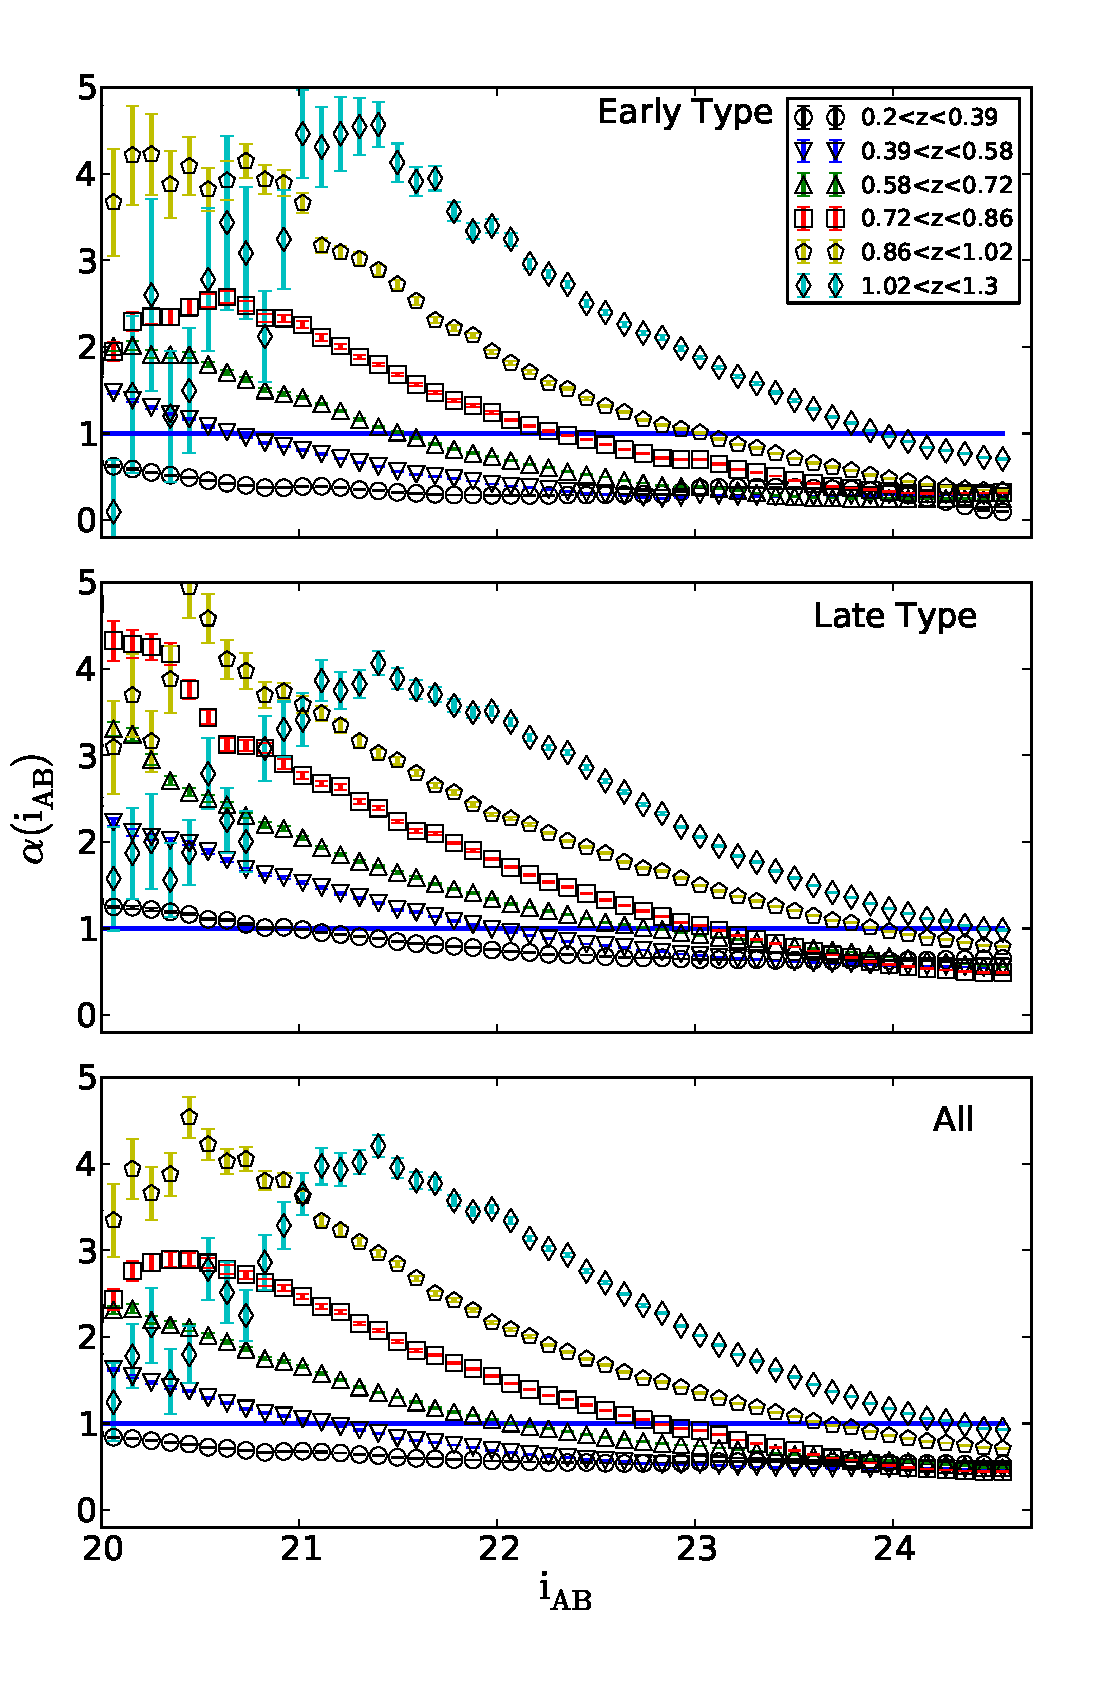
\includegraphics[width = 0.5\textwidth]{Alpha_Early_Late_All.pdf}
\caption{The slope of the cumulative galaxy number counts, $\alpha$,  as a function of magnitude for a sample of redshift bins, chosen to as the set of tomographic bins used in \citet{Heymans:2013p2015}, for a population consisting of early type galaxies (upper), late type galaxies (middle) and the full combined sample (All)(lower). } \label{fig:Alpha_Mag_Redshift}
\end{figure}



We construct the cumulative number densities of galaxies as a function of limiting magnitude, where sources have been separated into redshift bins, and take the slope of the cumulative number counts as set out in Equation \ref{Eqn:Alpha_Magnitude} to calculate $\alpha$.  Figure \ref{fig:Alpha_Mag_Redshift} shows $\alpha$ as a function of magnitude limit for six tomographic redshift bins as used in \cite{Heymans:2013p2015} for three sets of galaxy samples split by population type according to their spectral energy distribution (SED) template value ($T$): early type galaxies characterised by $T\ge2$, late types taken to have $2\le T$, and a full sample (labelled ``All''). Errors are taken from a bootstrap analysis, and agree with the estimated errors taking the variance of $\alpha$ across all fields. 

Whilst the value of $\alpha$ varies across the range of limiting magnitudes, all redshift bins converge to a similar value near the limiting magnitude of CFHTLenS at $i_{\rm AB} = 24.7$. The maximum value of $\alpha$ may occur at lower magnitudes. However, by cutting at lower magnitudes, we reduce the number of galaxies in the sample thus increasing the shot noise contribution. This suggests that choosing a magnitude cut to maximise $\alpha$ and consequently the strength of the contribution magnification to the clustering signal may not maximise the signal to noise. 

We therefore define a signal-to-noise estimate for background redshift bin $(j)$ lensed by foreground redshift bin $(1)$ as
\be\label{eqn:SignalToNoiseEst}
\hat{S}^{(j)}(i_{\rm AB}) = \langle n^{(1)} \rangle \langle n^{(j)}(i_{\rm AB})\rangle[\alpha^{(j)}(i_{\rm AB})-1]^2,
\ee
where the magnitude limit for the foreground bin is chosen to be as deep as possible to maximise $\langle n^{(1)}\rangle$. The signal to noise estimator $\hat{S}$ is calculated using the magnification-intrinsic clustering power spectrum $P_{gm}$ as the data, is proportional to the square of the true signal-to-noise, and cosmic variance is been assumed to be a subdominant contribution to the noise. %By maximising $\hat{S}$ we therefore maximise the contribution of the magnification-intrinsic clustering power spectrum $P_{gm}$ to the total power defined in Equation \ref{eqn:NumberDensityContrastPS}, therefore maximising the sensitivity of the data to magnification bias, as can be seen by noting that $P_{mg}>P_{mm}$ on all scales (Figure \ref{Fig:NumberPowerSpectra}). 
Figure \ref{Fig:SignalToNoise} shows how $\hat{S}$, rescaled by the maximum signal-to-noise at the limiting magnitude of the survey, behaves as a function of limiting $i$ magnitude, for early and late type galaxy subsamples. 

We see from Figure \ref{fig:Alpha_Mag_Redshift} that there is little variation in $\alpha$ between samples chosen to contain early or late type galaxies, with the value for $\alpha$ at a given magnitude limit and redshift bin typically larger for late type galaxies. As the catalogues used contain predominantly late type galaxies, the behaviour of $\alpha$ as a function of magnitude in the full sample is set mainly by the late type galaxies, and similarly for the signal to noise estimator. Whilst the difference in $\alpha$ values between late and early type samples are small, the difference between the two samples is more noticeable in their respective signal to noise values. Typically, the signal to noise for the late type galaxies are larger than those for the early type subsample, and this can be attributed to the fact that the late type subsample contains more galaxies thus reducing the shot noise contribution. %For the same reason, the signal to noise for the full sample is typically larger for all redshift bins than both the early and late type subsamples. 

\begin{figure}
\centering
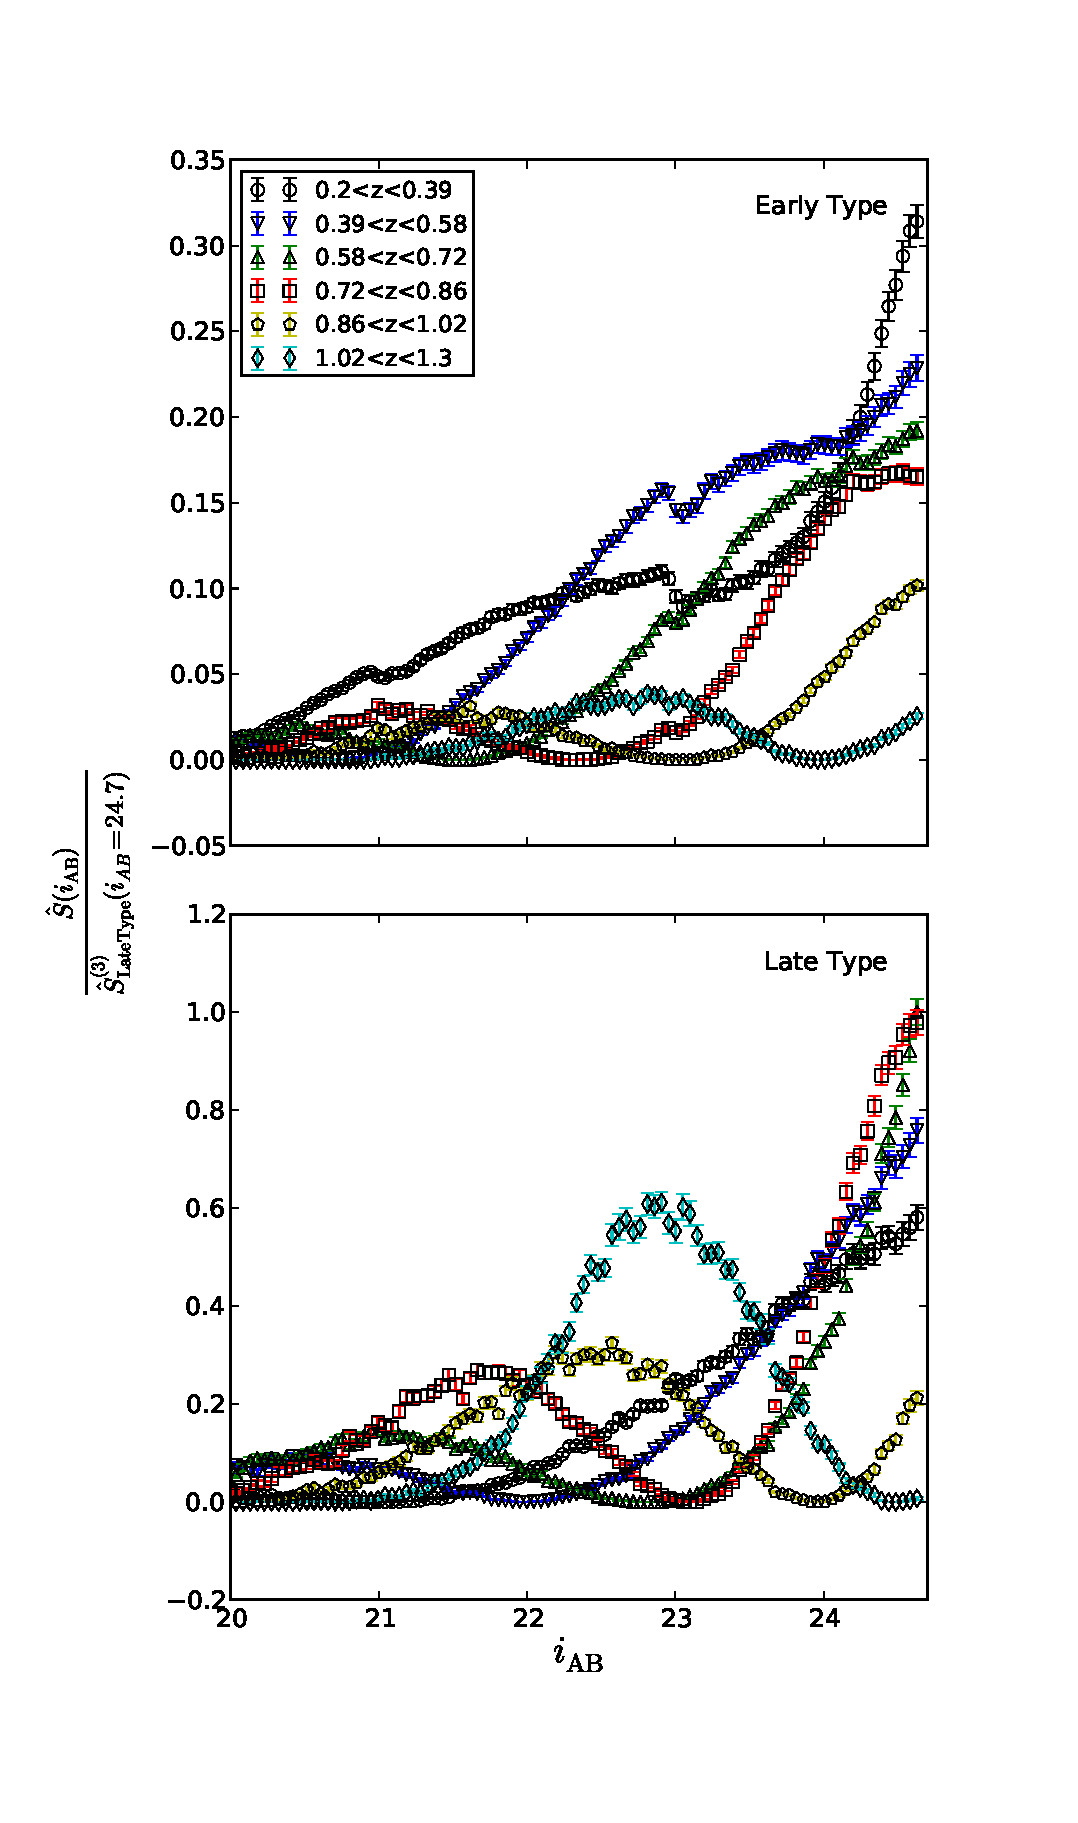
\includegraphics[width = 0.5\textwidth]{SignalToNoise.pdf}
\caption{The signal-to-noise estimator $\hat{S}$ as a function of magnitude for a sample of redshift bins, chosen as the set of tomographic bins used in \citet{Heymans:2013p2015}, for a population consisting of Early Type galaxies, and Late Type galaxies. To aid comparison, signal-to-noise values are rescaled to the maximum signal-to-noise value at the magnitude limit of the survey, which occurs in the redshift bin $3$, $0.58<z<0.72$ in the late type subsample. The signal-to-noise for the late type subsample is typically larger than the early type subsample, which can be attributed to the smaller early type population in the full catalogues. The reader should note that each axis plotted with different scaling of the y-axis.}\label{Fig:SignalToNoise}
\end{figure}

For the late type subsample, all redshift bins show an oscillation in signal-to-noise at lower magnitude limits. These oscillations occur due to the interplay in the reduction in noise by adding more galaxies to the sample as we cut a fainter magnitudes, and the increase in strength of the magnification bias as the sample is chosen to maximise the number of galaxies brought into the survey over this flux limit. For all redshift bins, we therefore see an increase in the signal-to-noise as the noise is reduced by increasing the size of the sample, followed by a reduction in signal-to-noise as $\alpha\to 1$ and there is no change in number density contrast due to magnification bias. Finally, past this limit and for $\alpha < 1$ the reduction in noise from increased sample size causes a final increase in the signal-to-noise. 

For the redshift bins encompassing $0.2\le z<0.86$ the peak of the signal-to-noise estimator at the faint limit of the survey ($i_{\rm AB} = 24.7$) is larger than the peak of the oscillation for each respective redshift bin, however in the two largest redshifts bins, the peaks of these oscillations give a larger signal-to-noise at a lower magnitude than that obtained by naively cutting at the faint limit of the survey. This suggests an analysis chosen to optimise the strength of the magnification contribution to the measured clustering power spectrum should cut at these lower magnitude limits for these redshift bins, however they only occur for the highest redshift bins for which photometry is least accurate, and are nearly entirely absent in the early type subsample. 


As well as adding galaxies at the faint end of the luminosity function, magnification should also remove galaxies at the bright end of the luminosity function. Assuming that all galaxies in a redshift bin experience an increase in magnitude $\Delta i_{\rm AB}$ as a result of lensing by the foreground, then the number of galaxies removed at the faint end is roughly $N(<m_{faint})\Delta m$, whilst those removed at the bright end are $\sim N(<m_{bright})\Delta m$ \footnote{This ignores the second order effect of the change in the cumulative number of sources brighter than the faint end by the removal of sources at the bright end}. Provided $N(<m_{bright})/N(<m_{faint})\ll1$, we expect the effect of the removal of sources at the bright end to be subdominant, and ignore it. By choosing a magnitude cut close to the bright limit, this effect becomes more important. 

For these reasons, we limit the choice of $\alpha$ values only to values close to the faint limit of the survey, and consider $0<\alpha<4$ as reasonable. Unless otherwise stated, results are shown assuming $\alpha = \ATrue$ across all redshift bins, which is the value calculated for the full galaxy sample for $i_{\rm AB}\le 24.7$ and $z\le 0.86$.

\subsection{Survey modelling}\label{Sec:SurveyModelling}

In this analysis, we consider two types of survey, following a Dark Energy Task Force-like classification of surveys considering
\begin{enumerate}
\item{A Stage III ground-based survey (hereafter S3), covering $1500\:{\rm deg}^2$ to a depth of $i_{\rm AB} = 24$. Sources are measured between photometric redshift limits  $z_{\rm Phot} = (0,2)$ with photometric redshift errors $\sigma_{\rm Phot} = 0.05(1+z_{\rm Phot})$}
\item{A Stage IV space-based survey (hereafter S4), which covers $15,000 \:{\rm deg}^2$ of the sky, to a depth of 24.7 in the $i$-band, between photometric redshift limits $z_{\rm Phot} = (0,2)$, and with photometric redshift errors $\sigma_{\rm Phot} = 0.05(1+z_{\rm Phot})$. Unless otherwise stated, results hereafter are shown for an S4 survey.}
\end{enumerate}

The matter power spectrum is modelled using \cite{Eisenstein:1998p1135} transfer functions with \cite{Smith:2003p843} non-linear corrections.

Figure \ref{Fig:CFHT_Neff_Zmed} shows the median survey redshift, and effective number density of galaxies as a function of faint limiting $i_{\rm AB}$ magnitude taken from CFHTLenS catalogues for galaxies with valid shape measurement as well as for all galaxies with photometry. From this we choose for our S3 survey a median redshift of $z_{\rm med} = 0.66$, and galaxy number density of $\langle n\rangle = 8.5 \;{\rm gal/arcminute}^2$ and $18\;{\rm gal/arcminute}^2$ for an shear analysis, and clustering analysis respectively.  Similarly, we consider for an S4 survey $z_{\rm med} = 0.7$, however on choosing a global number density of sources we consider the case where shapes can be measured for every photometric source. Therefore, we use the photometry line in deducing the number density of galaxies for S4, and take $n_{\rm gal} = 28\;{\rm gal/arcminute}^2$ for both shear and clustering analyses.  

\begin{figure}
%\centering
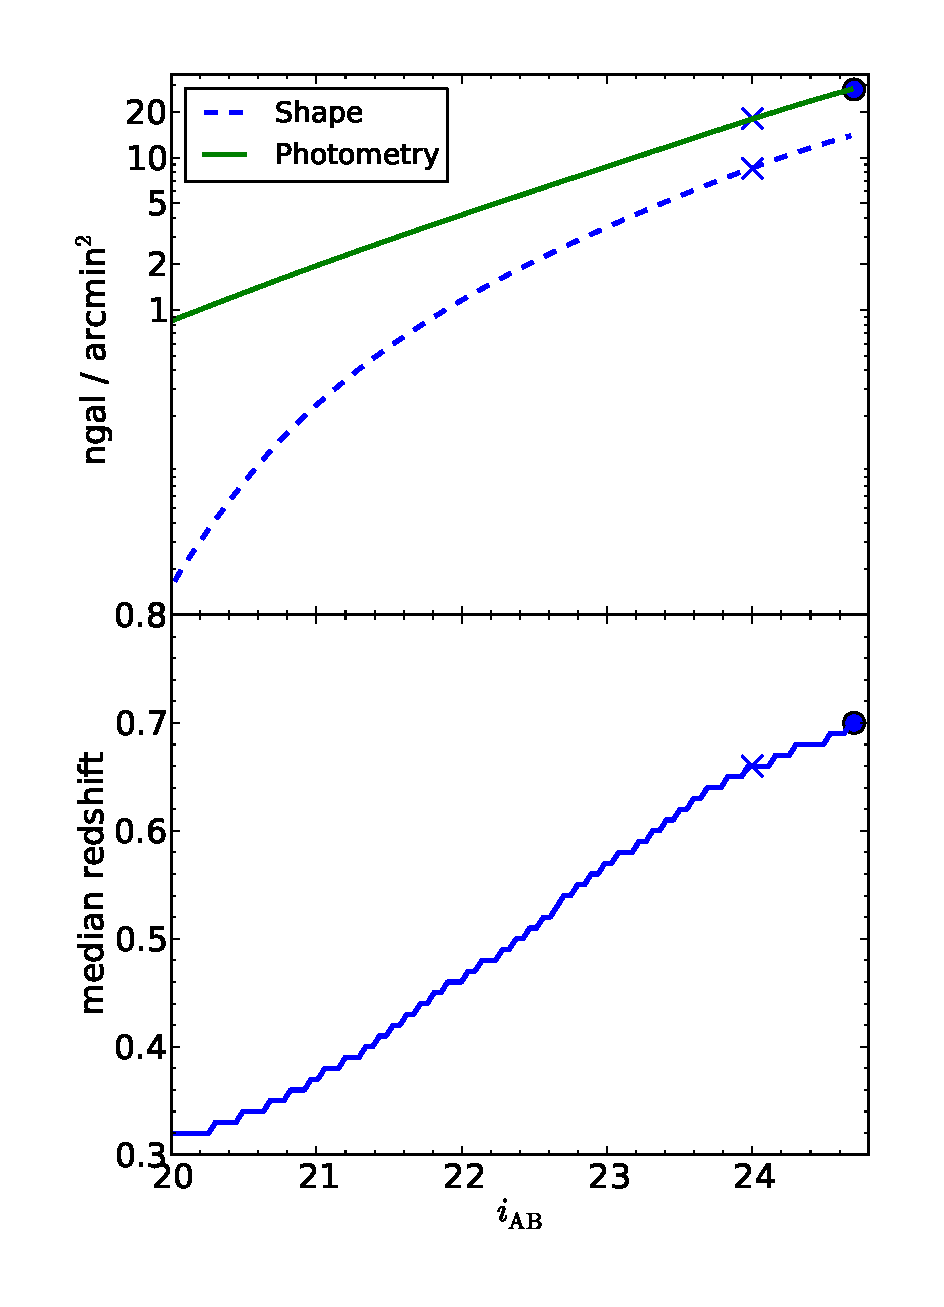
\includegraphics[width = 0.5\textwidth]{neff_zmed.pdf}
\caption{The top panel shows the effective number density of galaxies (in gal/arcminute$^2$) as a function of faint limiting magnitude $i_{\rm AB} $for sources with valid shape measurement (dashed), and all galaxies with photometry (solid). The bottom panel shows the median redshift of sources as a function of limiting magnitude. All data is taken from CFHTLenS catalogues. Crosses mark values taken for our S3 survey model, whilst dots mark values take for our S4 survey model.}\label{Fig:CFHT_Neff_Zmed}
\end{figure}

\subsection{Galaxy redshift distributions}\label{Sec:Galaxy_Redshift_Distributions}

We model the galaxy distributions of true redshift as
\be
p^{(i)}(z_{\rm t}) = \int_{z^{(i)}_l}^{z^{(i)}_h} dz_{\rm ph}\; p(z_{\rm t}|z_{\rm ph})p(z_{\rm ph})
\ee
where $p(z_{\rm t}|z_{\rm ph})$ is described by a Gaussian with width $\sigma_z = 0.05(1+z_{\rm ph})$ which describes the photometric redshift errors, and $z_l$ and $z_h$ denote the lower and higher bounds of the redshift bin in photometric redshift.  We model the galaxy redshift distribution as measured for photometric redshift, $p(z_{\rm ph})$, as \citep{Smail:1994p986}
\be
p(z_{\rm ph}) \propto \left(\frac{z_{\rm ph}}{z_0}\right)^{2.0}\exp^{-\left(\frac{z_{\rm ph}}{z_0}\right)^1.5}
\ee
with characteristic redshift $z_0$ related to the median redshift of the survey by $z_0 = z_{\rm med}/1.412$. The galaxy redshift distribution is subdivided into redshift bins such that each bin contains the same number of galaxies. 

Figure \ref{Fig:Distributions} shows the resultant galaxy distribution for 8 redshift bins for survey types S3 and S4, with the resultant number density contrast power spectra given for three choices of bin combination in Figure \ref{Fig:NumberPowerSpectra}. Noticeably, for closely separated redshift bins, the intrinsic clustering term is non-vanishing due to the presence of photometric redshift errors which cause some galaxies to be incorrectly assigned to a given redshift bin, and causes overlap between the binned galaxy distributions, and the intrinsic clustering-magnification cross term is always dominant over the pure magnification power spectra. As we take redshift bins that are more widely separated, the power from intrinsic clustering decreases, so we see that for the most widely separated bins the total power is dominated by terms that include the magnification. As the cross power is always dominant to the pure magnification power, frequently studies will ignore the pure magnification contribution to the overall clustering power, and instead just quote the cross contribution, usually in the situation where correlations are considered between distant foreground and backgrounds, so the intrinsic clustering contribution is subdominant and may also be ignored. In this analysis, we consider all contributions to the power, as given in Equation \ref{eqn:NumberDensityContrastPS}.

%We account for this change in sample size by considering a change in the signal to noise cut in flux, above which galaxies are included in the sample, and which corresponds to a change in the maximum magnitude to which galaxies are included. Using CFHTLenS catalogues (described in Section \ref{Sec:CFHT}), we determine the following relations between the median redshift of the sample and the number density of sources in the sample
%\be\label{eqn:Median_Redshift_Fit}
%\Delta z_{med} = 0.07\Delta M  %z_{med} = 0.07(M - 17.4) 
%\ee
%with $\Delta M = M^{\delta n} - M^{\kappa_s}$, $M$ denotes the magnitude cut, and $\Delta z_{med} = z_{med}^{\delta n} - z_{med}^{\kappa_s}$, and
%\be
%n_g = n_g^{\kappa_s}\left(\frac{z_{med}^{\delta n}}{z_{med}^{\kappa_s}}\right)^{5}.
%\ee
%A difference in signal to noise cuts of $2.5$ in flux corresponds to a magnitude limit difference of $\sim 1$, giving a difference in the median redshift of the measured galaxy distribution in photometric redshifts of $0.07$ by Equation \ref{eqn:Median_Redshift_Fit}. The renormalised convolved galaxy distributions in spectroscopic redshifts used for the shear and clustering signal are shown in Figure \ref{fig:SpecRedshiftDist}, where the modelled redshift distribution for the sample used for the clustering signal probes deeper in redshift than that of the shear.

\begin{figure}
%\centering
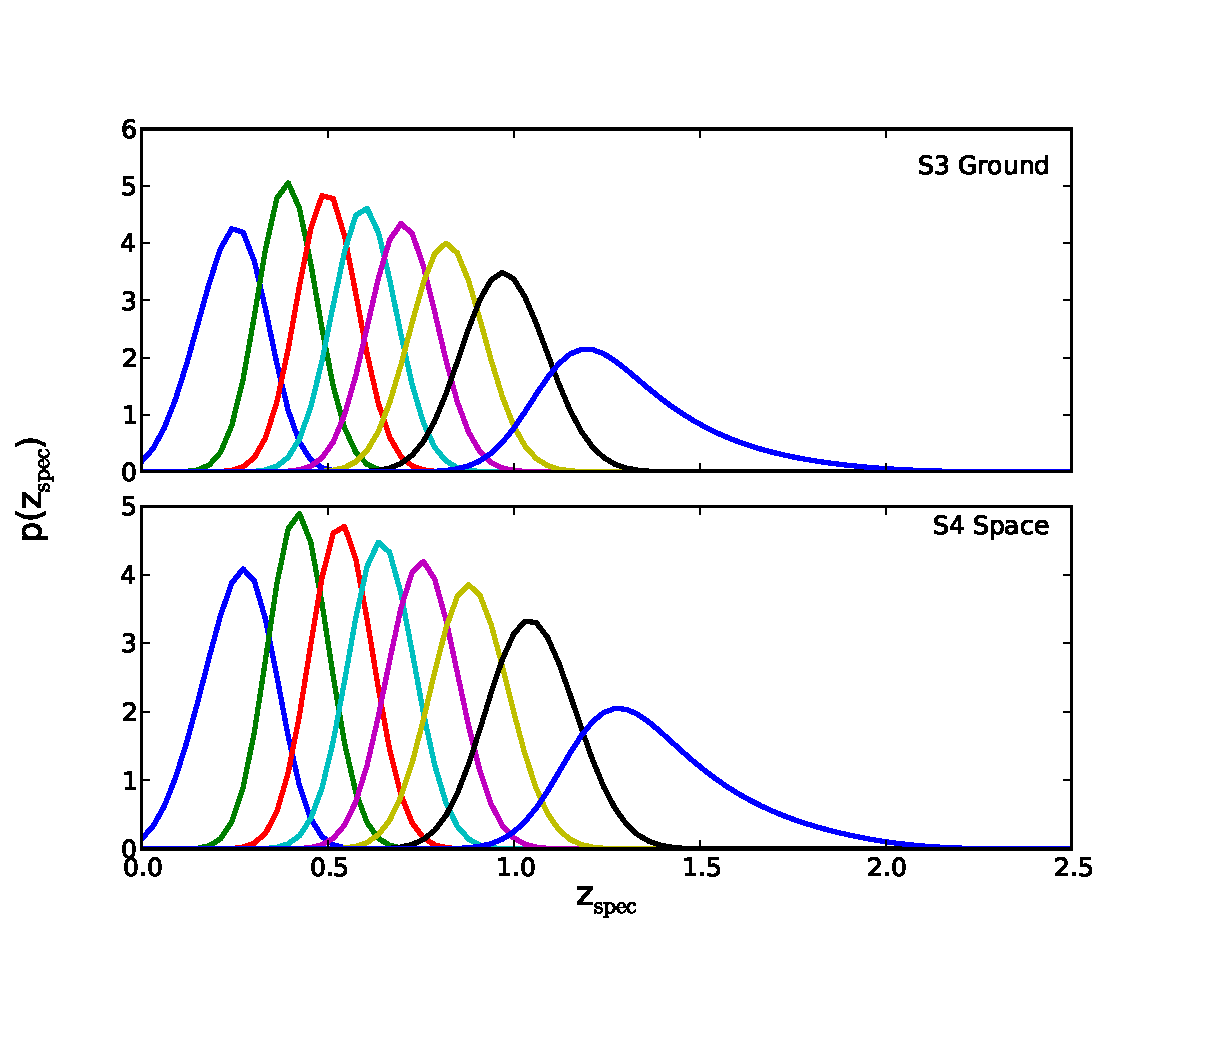
\includegraphics[width = 0.5\textwidth]{Distributions_Surveys.pdf}
\caption{Galaxy redshift distributions as defined in Section \ref{Sec:Galaxy_Redshift_Distributions}, for an S3 ground-based (top) and S4 space-based (bottom) survey (defined in Section \ref{Sec:SurveyModelling}). Each redshift bin has been renormalised so that $\int dz \; p^{(i)}(z) = 1$. }\label{fig:SpecRedshiftDist}\label{Fig:Distributions}
\end{figure}

\begin{figure}
\centering
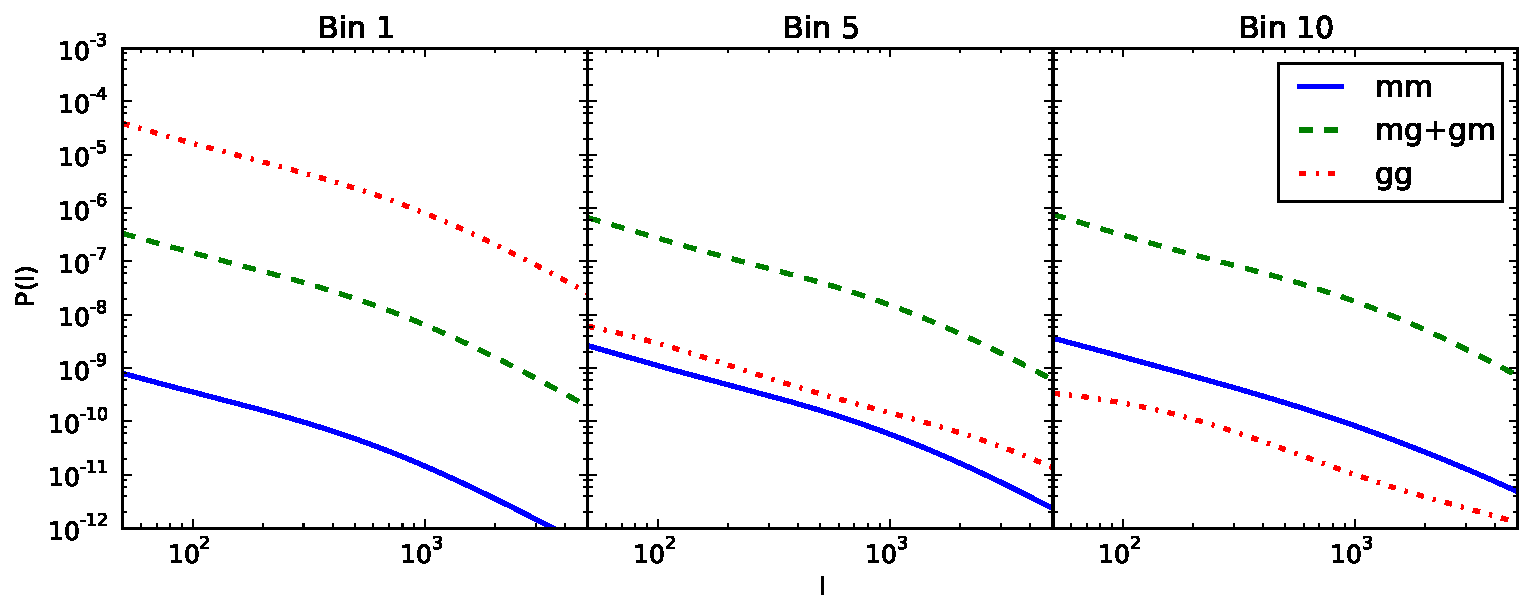
\includegraphics[width = 0.47\textwidth]{PS.pdf}
\caption{Contributions to the number density contrast power spectrum for a combination of background redshift bins, for the S4 binned galaxy distribution functions given in Figure \ref{Fig:Distributions}. The foreground bin is chosen to be redshift bin $1$. It can be seen that for foreground and background that are spatially close in redshift, the overlap in redshift distribution due to redshift errors can easily cause the magnification terms (mg or mm) to be swamped by the intrinsic clustering term (gg). As we increase the separation in redshift between foreground and background, the amplitude of the gg term decreases whilst the cross (mg + gm) and mm term increase.} \label{Fig:NumberPowerSpectra}
\end{figure}

\section{Results}\label{Sec:Results}

\subsection{The effect of galaxy bias}
In this section, we present forecasts for our S3 and S4 survey models, using the Fisher matrix formalism set out in Section \ref{Sec:FM_Clustering_All}. We first investigate the effect of galaxy bias on the constraining power from a clustering analysis including magnification bias, when all redshift bin combinations are used. Figure \ref{Fig:Contours_M_K} shows contours for the set of cosmological parameters laid out in Section \ref{Sec:ParameterForecasts}, for the cases where we consider constraints coming from only galaxy ellipticites, or number density contrasts only.  Figure \ref{Fig:Contours_MK_K_MargFixed} shows $1-\sigma$ parameter constraints for a shear only analysis, and a combined shear and clustering analysis . For analyses that contain number density contrast as a probe, $\ell$-cuts are applied and galaxy bias is either marginalised over, meaning that it is constrained simultaneously to cosmological parameters from the number density contrast signal (labelled as unknown galaxy bias), or fixed to $b = 1$ (labelled as known galaxy bias). 

It is evident that in the case where galaxy bias is known, constraints from a clustering analysis are competitive to cosmic shear, however when galaxy bias is unknown and must also be constrained from the data the constraints from clustering are much weaker. This is expected, as when the linear galaxy bias is known the intrinsic clustering contribution to the power spectrum directly probes the matter power spectrum. 

\begin{figure*}
\centering
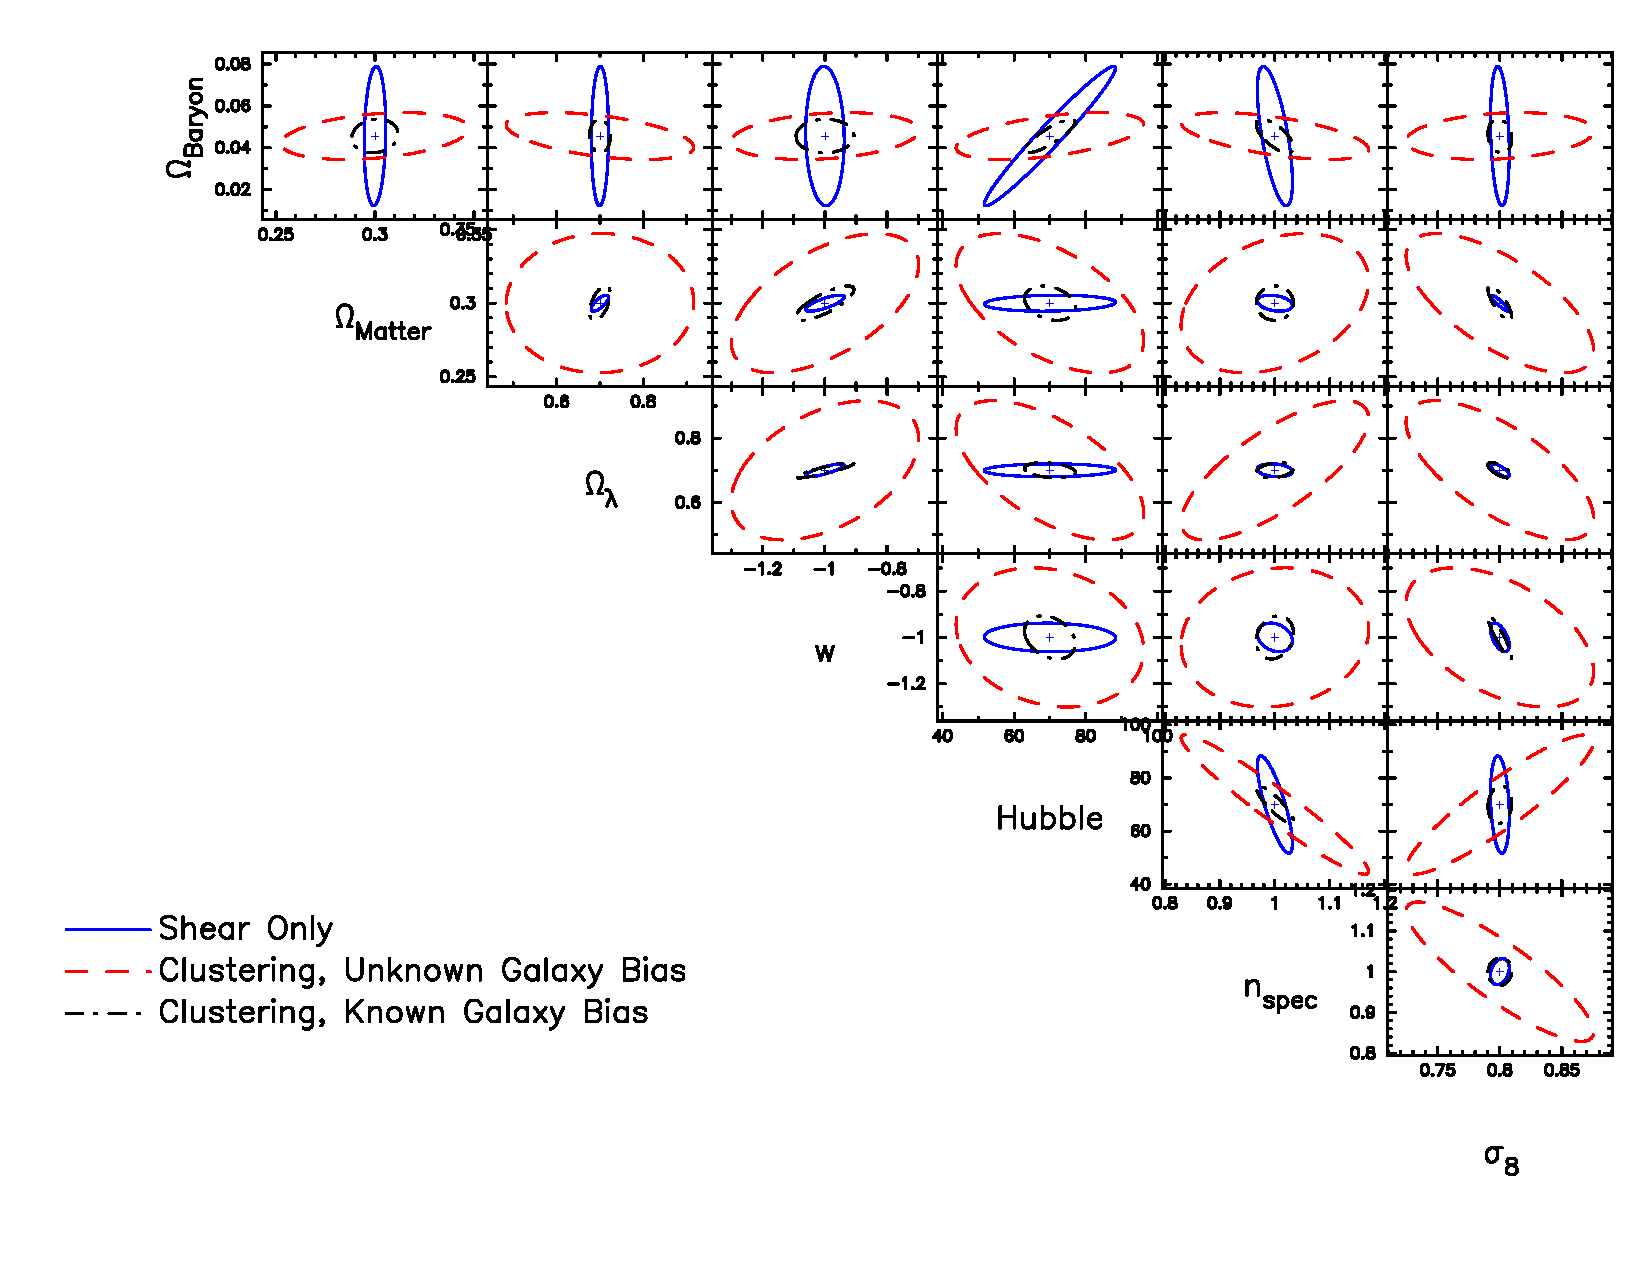
\includegraphics[scale=0.65]{Contours_M_K.pdf}
\caption{Fisher matrix forecast showing $1-\sigma$ constraints of cosmological parameters for an S4 space-based survey, considering measurements of galaxy ellipticities only (``shear only'', solid blue line), and galaxy clustering including magnification bias where the galaxy bias is known and taken to be $b = 1$ (black dot-dashed) or unknown and simultaneously constrained with the data (red dashed). Constraints from clustering with magnification bias assume $\alpha = \ATrue$, and only contain data from linear scales. Cuts on $\ell$-modes are applied as detailed in Section \ref{Sec:GalaxyBiasModelling}, with $\sigma_R < 0.5$. }\label{Fig:Contours_M_K}
\end{figure*}

It is worth noting that constraints from clustering only on $\Omega_{B}$ and $h$ are competitive to ellipticity measurements, as the clustering data can pick out the turnover in the matter power spectrum better than ellipticity measurements, as the kernel for projected number density fluctuations (Equation \ref{eqn:Projected_NumberDensity}) is much narrower than that for cosmic shear (Equation \ref{eqn:ProjectedConvergence}). Whilst seemingly promising, distance probes combined with CMB measurements will also constrain these parameters very well.

When we consider the case where a combined analysis is used, we see that there can be a significant improvement when adding number density contrast data to ellipticity measurement, however the improvement to constraints on cosmological parameters is strongly dependent on whether galaxy bias is constrained using the data, or set to a fixed known value (Figure \ref{Fig:Contours_MK_K_MargFixed}). In the case where galaxy bias is known there is a marked improvement to constraints, especially in the $\Omega_M - \sigma_8$ plane. This is in agreement with the results of \cite{VanWaerbeke:2010p8}, in which galaxy bias was assumed linear and fixed to $b=1$, however we see that when galaxy bias is unknown much of the additional constraining power from clustering is lost, and thus we conclude that the constraints presented in \cite{VanWaerbeke:2010p8} will be too optimistic. 

\begin{figure*}
\centering
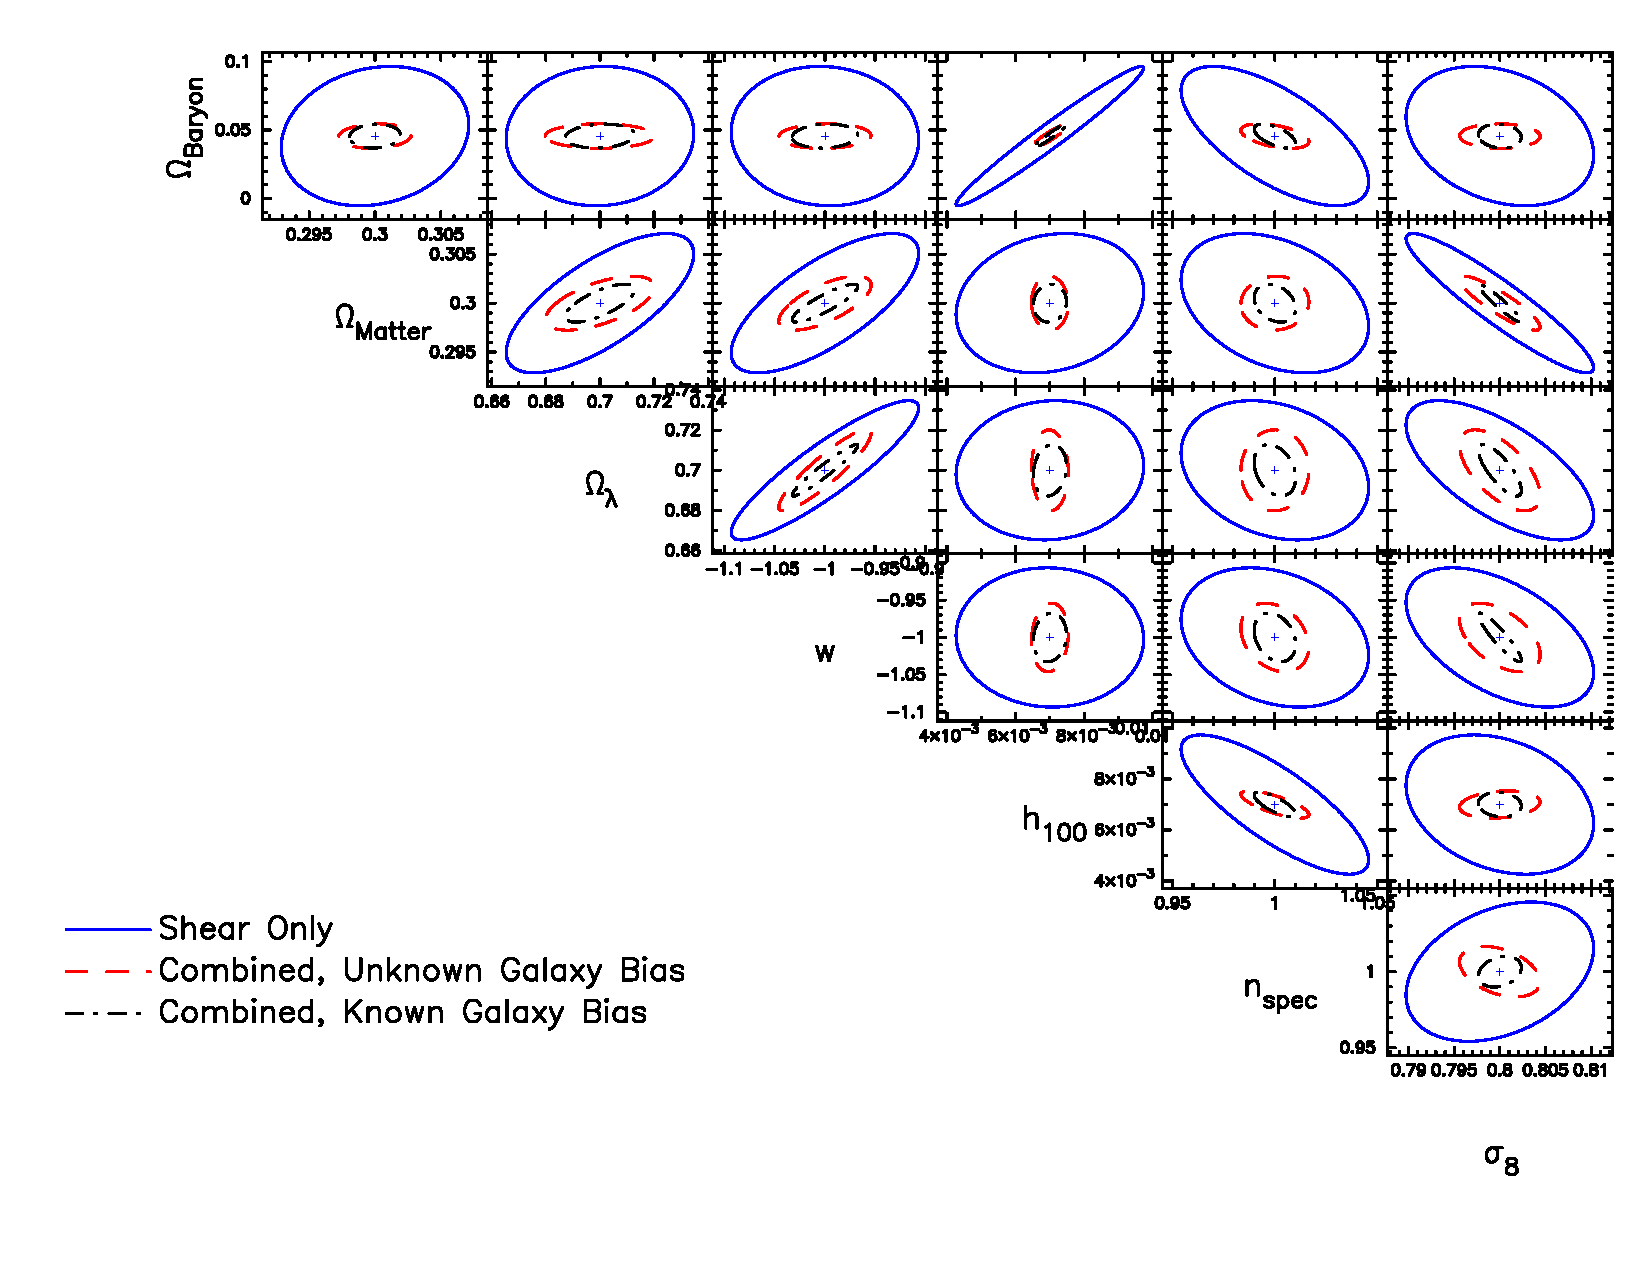
\includegraphics[scale=0.65]{Contours_MK_K_FixedMargGBias_S4.pdf}
\caption{As Figure \ref{Fig:Contours_M_K}, but instead comparing measurements from galaxy ellipticities only (``shear only'', solid), with a combination of shear and galaxy clustering measurements for known galaxy bias, $b=1$, (dot-dashed), and unknown galaxy bias which is simultaneously constrained by the data (dashed)}\label{Fig:Contours_MK_K_MargFixed}
\end{figure*}

We note however that even when the galaxy bias is unknown and simultaneously constrained with the clustering data, information from galaxy clustering can significantly improve cosmological parameter constraints from shear alone, corresponding to an increase by $3.58$, and $5.37$ to FoM$_{\rm DE}$ and FoM$_{\rm Cos}$ respectively from their values when using shear only. However when more conservative cuts on $\ell$-modes are used to exclude more non-linear scales, much of this extra information is lost. Whilst in this analysis we consider only scales below which $\sigma_R < 0.5$, as detailed in Section \ref{Sec:GalaxyBiasModelling}, we note that choosing $\sigma_R < 0.2$ causes an increase by $1.76$ and $3.1$ to FoM$_{\rm DE}$ and FoM$_{\rm Cos}$ respectively from their values when using shear only. We draw similar conclusions for the S3 model, with improvements to FoM values by a factor of $6.27$ and $10.38$ when clustering using all redshift bins is added to the shear analysis, with $\sigma_R<0.5$. The larger improvement from a combined analysis over shear only in this case due to decrease in shot noise in the clustering correlations, as the photometric sample is larger than the shape sample.		

Finally, whilst considering fully known and unknown galaxy bias gives us useful limits on the information gain from combining number density contrast measurements with ellipticity considerations, it may be expected that a more realistic version lies somewhere between the two, especially if galaxy bias can be constrained externally. Therefore, we consider how much information can be regained by correlating galaxy bias parameters across redshift bins, equivalent to making the galaxy bias a smooth function of redshift, or limiting it's uncertainty using an external probe, by the addition of a prior on galaxy bias of the form detailed in Section \ref{Sec:GalaxyBiasModelling}. Figure \ref{Fig:BiasPrior_ContourPlot} shows $\rm{FoM_{Cos}}$, defined in Section \ref{Sec:ParameterForecasts}, for a range of correlation strengths and uncertainties. It is evident that the uncertainty in galaxy bias is dominant in the recovery of information, however there is a weak improvement of Figure of Merit when the correlation strength is increased. %Conclusion to this? Get r values form some technique and feed in?

In \cite{Gaztanaga:2012p1194}, the authors conclude that magnification alone can produce better results than shear alone when the galaxy bias is known, however the reader must note that the authors use magnification is the same way that we use the term clustering in this work, using all contributions to number density fluctuations including intrinsic clustering over all redshift bin combinations. Accounting for the fact that we use different definitions for our figure of merits, our results seem to be in good agreement with those presented therein. It should be noted, however that the authors of \cite{Gaztanaga:2012p1194} choose much more optimistic $\ell$-cuts than those presented here, and apply these $\ell$-cuts to all probes including their shear measurements. In addition, the authors also use only linear theory when modelling the matter power spectrum , suggesting they should over-estimate constraints from galaxy clustering whilst under-estimating cosmic shear. Additionally, the authors model galaxy bias using four free parameters, whereas we assign a galaxy bias nuisance parameter to each redshift bin used.

As a result, the authors of \cite{Gaztanaga:2012p1194} find that clustering (or magnification in their terminology) with unknown galaxy bias is much more competitive with cosmic shear than we find in this work, however we both find that when galaxy bias is known that galaxy clustering can be a competitive probe of cosmology to cosmic shear alone.  Similarly, we both find that the combination of galaxy clustering, galaxy-galaxy lensing and cosmic shear gives a significant improvement to statistical errors on cosmological parameters than an analysis using cosmic shear alone.


%\begin{figure*}
%\centering
%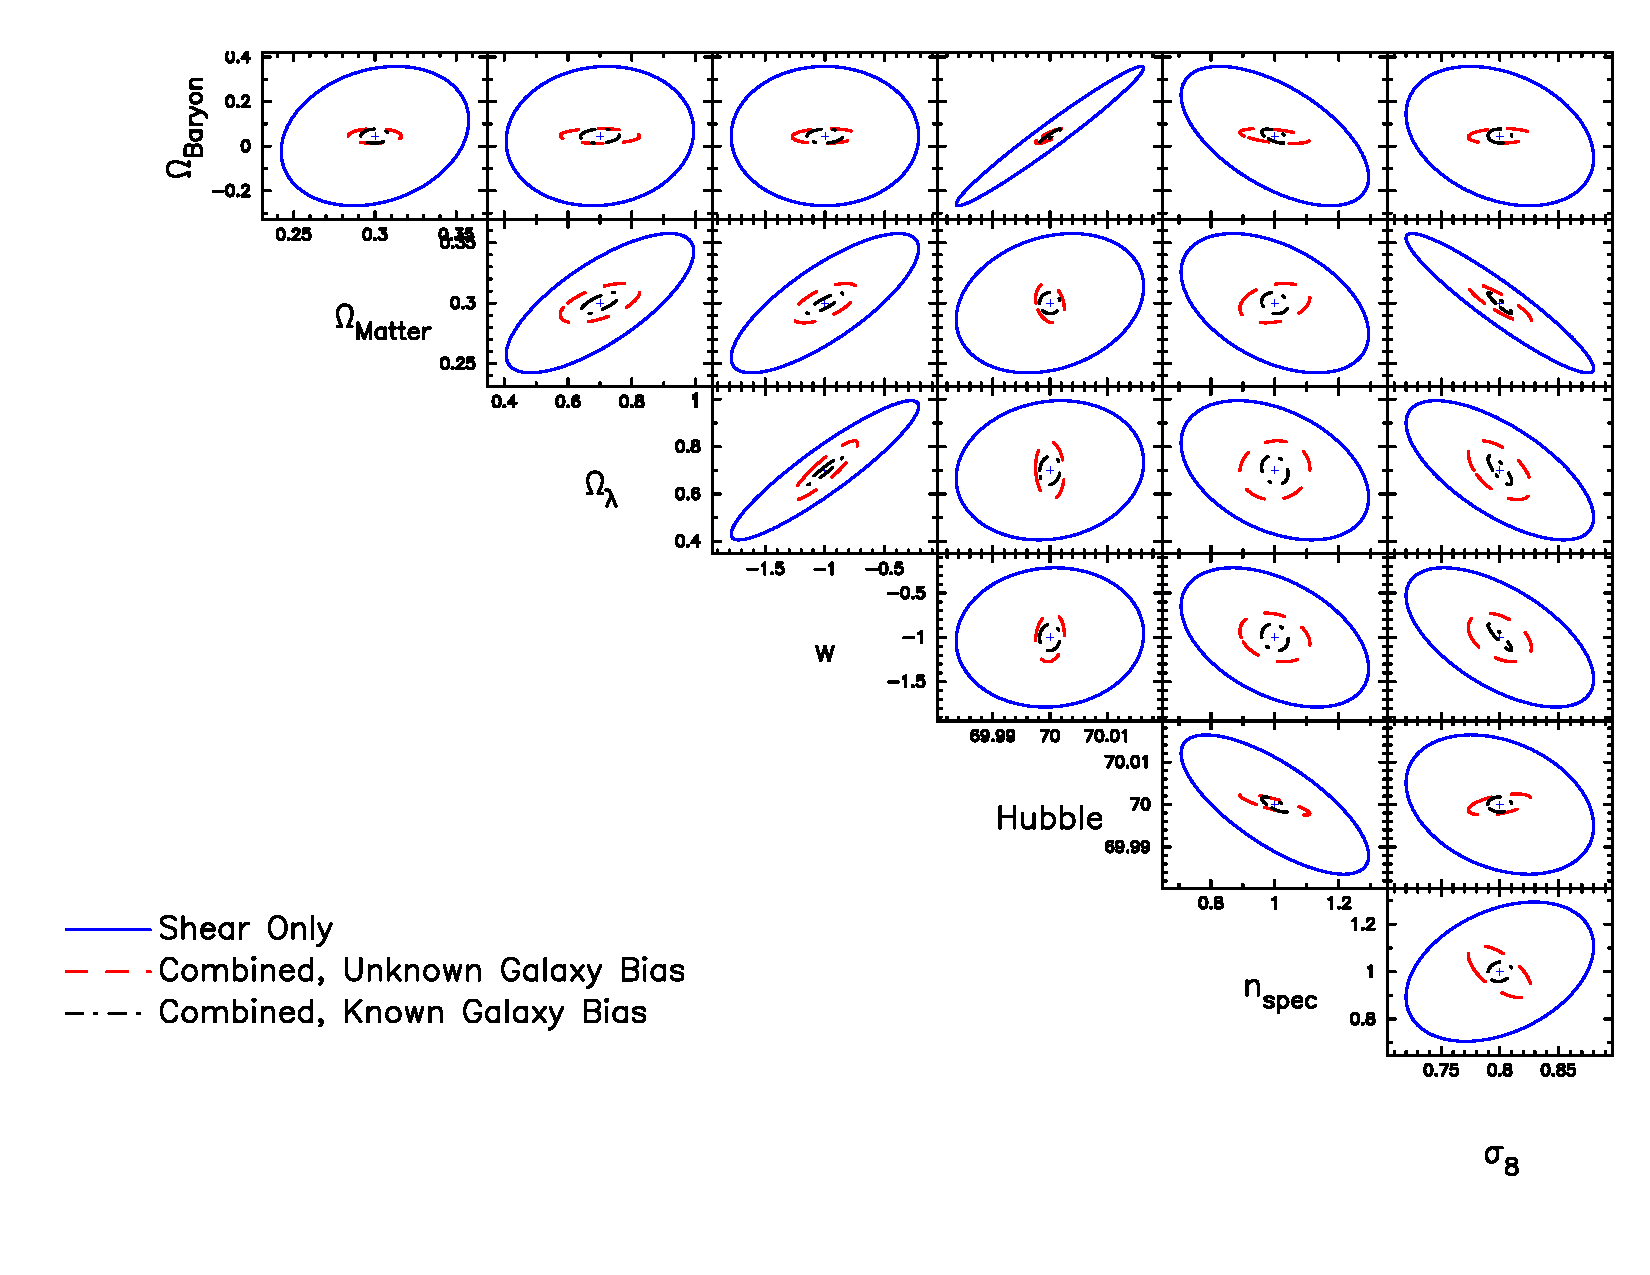
\includegraphics[scale=0.65]{Contours_MK_K_FixedMargGBias_S3.pdf}
%\caption{Contour plot for magnification signal showing a shear analysis, and combined shear and clustering analysis taking a known and fully unknown galaxy bias, for an S3 ground-based survey.}\label{Fig:Contours_MK_K_MargFixed_S3}
%\end{figure*}

\begin{figure}
\centering
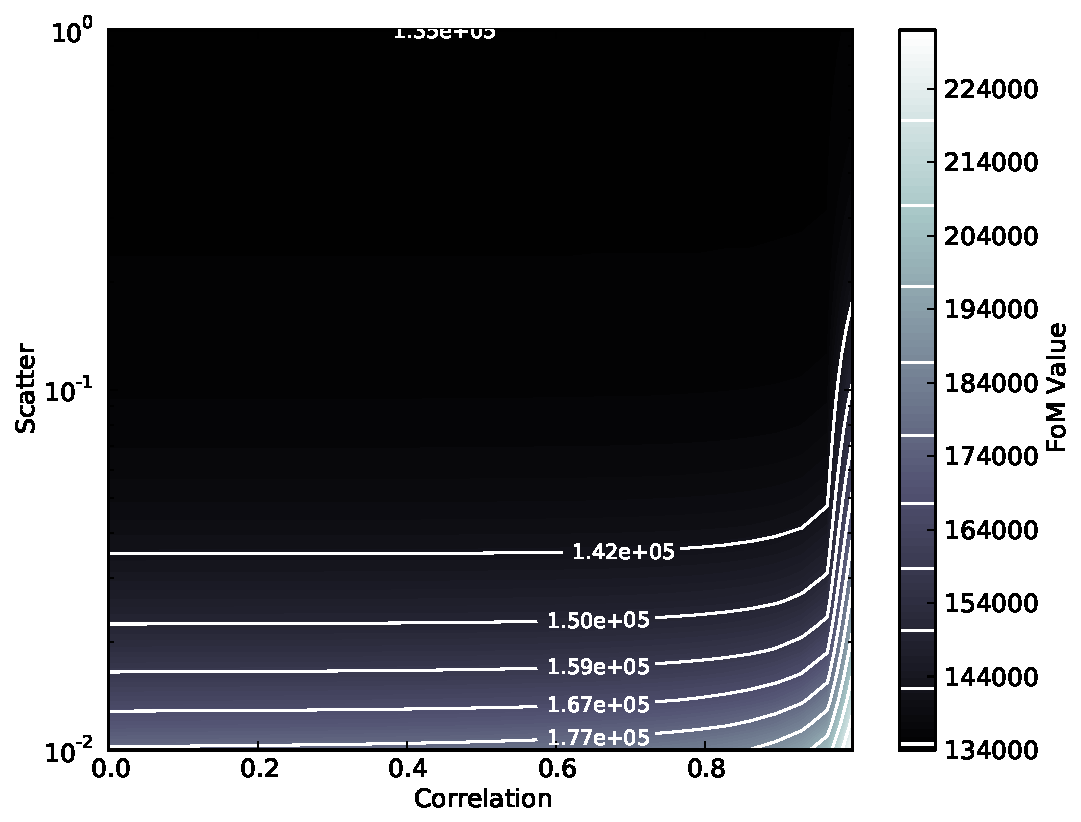
\includegraphics[width = 0.5\textwidth]{BiasPriorLoop_FoM.pdf}
\caption{Contour plot showing constant-FoM$_{\rm Cos}$ contours as a function of $\sigma$ and $r$ ( the uncertainty and correlation in Bias Prior as detailed in Equation \ref{Eqn:BiasPriorCov}). }\label{Fig:BiasPrior_ContourPlot}
\end{figure}


\subsection{The contribution from magnification bias}\label{Sec:Constraints_AlphaDependance}

In this section, we question just how much of the constraining power using the number density contrast comes from the magnification terms ($P_{mm}, P_{mg}+P_{gm} $ in Equation \ref{eqn:NumberDensityContrastPS}), and how much can be obtained from the intrinsic clustering only ($P_{gg}$). If $\alpha = 1$, the terms which depend on the magnification are identically zero, so that number density fluctuations come from the intrinsic clustering of galaxies only, and in the limit of large $\alpha$, the number density contrast power spectrum is dominated by the magnification only contribution ($P_{mm}$) for all redshift bin combinations. By altering $\alpha$, we can therefore alter the strength of the contribution from magnification, and therefore test the level of contribution to parameter constraints from the magnification effect.

Figure \ref{Fig:FoM_Alpha} shows the figure of merit (FoM$_{\rm Cos}$) as a function of $\alpha$ when considering galaxy clustering only as a probe, and when combining galaxy clustering measurements with cosmic shear measurements. We note that the FoM increases with as the contribution from magnification bias becomes larger, and the minimum in the FoM$_{\rm Cos}$ occurs when the $\alpha = 1$ and the contribution to the clustering powers spectrum from the magnification terms is zero. We can therefore conclude that a non-zero measurement of $\alpha-1$ will improve the total constraints on all cosmological parameters provided no galaxies are removed from the sample. However , as discussed in Section \ref{Sec:CFHT}, analyses that try to optimise for a clustering analysis by cutting at a magnitude limit which gives a large value of $\alpha$ may degrade the signal overall by removing sources from the sample and increasing noise.

Whilst similar behaviour is seen in the combined probe, we note that the relative improvement in the FoM as $|\alpha -1|>0$ is much smaller than the clustering only case. As the constraints on cosmological parameters from clustering are much smaller that those from shear when galaxy bias is unknown, most of the improvement in FoM by combining a shear and clustering analysis come from degeneracy breaking (see Figure \ref{Fig:Contours_M_K}), and so whilst a non-zero value of $\alpha$ may greatly improve the constraining power of a clustering only analysis, it does not change the constraining power of a combined clustering and shear analysis significantly. {\bf We note also that the minimum of FoM for the combined clustering and shear analysis does not lie at $\alpha  = 1$ as it does in the clustering only analysis. For $\alpha-1>0$, the magnification signal becomes more degenerate with the shear, and so we expect a shift in the minimum to slightly over $\alpha = 1$ for the combined analysis, over which the improvement to statistical errors from the clustering correlations due to an increase in $\alpha$ causes the FoM for the combined analysis to increase also.}

%The behaviour of FoM$_{\Omega_M,\sigma_8}$ from the combined probe is perhaps more surprising, as it shows a decrease in constraining power as $\alpha$ increases, and shows a maximum when $\alpha = 1$.  To understand this decrease in the figure of merit, consider the case when $\alpha \to 1$, and $\alpha \gg 1$: when $\alpha \gg 1$ the galaxy clustering power spectrum probes only the convergence power spectrum, $P_{mm} = 2(\alpha-1)P_{\kappa\kappa}$ term, and is therefore highly degenerate with the measurements of convergence through gravitational shear. In this case, we expect only a small improvement in cosmological constraints by combining both probes. However, when $\alpha \to 1$, the intrinsic clustering contribution becomes more dominant, which is less degenerate with the shear analysis, and therefore should improve constraints by degeneracy breaking.

%Figure \ref{Fig:FoM_Alpha} suggests that a non-zero magnification bias reduces the constraining power of a galaxy clustering analysis when combined with a shear analysis, however it should be noted that the change in FoM$_{\Omega_M,\sigma_8}$ is small as the strength of the magnification bias contribution is increased (a change of $\sim 3\%$ from $\alpha = 1$ to $\alpha = 3$). We can therefore conclude that the effect of the magnification bias terms on cosmological constraints is small. Figure \ref{Fig:Derivatives} shows the contribution to the derivatives of the galaxy clustering power spectrum with respect to $\Omega_M$ and $\sigma_8$ for each term defined in Equation \ref{eqn:NumberDensityContrastPS}. We see that for the redshift bin combinations where the power is dominated by the intrinsic clustering term, the derivatives with respect to cosmology are also dominated by the intrinsic clustering, suggesting that it is the intrinsic clustering contribution that is most sensitive to a change in cosmology. Of course, for large values of $\alpha$, both the power spectrum and derivatives become dominated by $P_{mm}$, however we note that for most cosmological parameters it takes unphysical values of $\alpha$ to achieve this (for example, for the derivative of $P_{mg} + P_{gm}$ with respect to $\sigma_8$ to become dominant in all redshift bins, we require $\alpha \sim 10$). We therefore conclude that for physically motivated values of $\alpha$, most of the constraining power comes from the intrinsic clustering contribution, even for the case where the galaxy bias is unknown and must be constrained simultaneously with the data. 

\begin{figure}
\centering
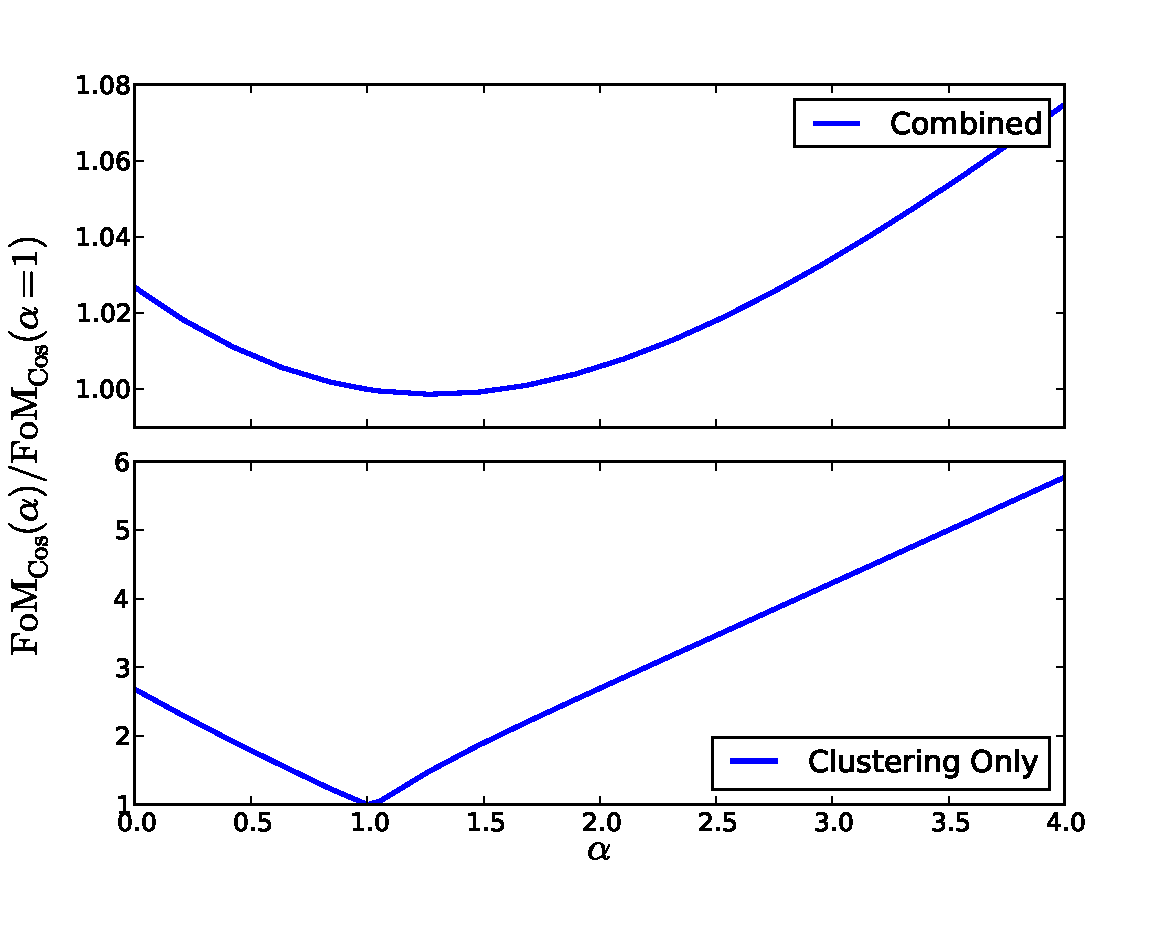
\includegraphics[width = 0.5\textwidth]{FoM_Alpha.pdf}
\caption{Figure of Merit (FoM$_{\rm Cos}$) as a function of $\alpha$ for a clustering only analysis (bottom), and combined shear and clustering analysis (top), for an S4 survey. All values are rescaled to the value of the figure of merit when $\alpha = 1$ corresponding to the case when fluctuations to the number density contrast come from the intrinsic clustering of galaxies only. Note the different scaling of the ordinate axis.}\label{Fig:FoM_Alpha}
\end{figure}

\subsection{Tomography}

We consider how much information can be gained from increasing the number of redshift bins we are considering in each respective analysis. Figure \ref{Fig:FoM_Nz} shows FoM$_{\rm Cos}$ as a function of $N_z$, the number of redshift bins, for cosmic shear, clustering analysis and a combined analysis. We see that for all three cases, the information gain by adding redshift bins is large for small numbers of redshift bins, but in all cases quickly asymptote to a constant. We note that for the shear only case, there is not much information gain in taking more than $\sim 4$ redshift bins, which agrees with results shown in \cite{Joachimi:2010p855}, however the clustering analysis continues to improve constraints up to much higher numbers of redshift bins, and only starts to asymptote to its maximum around $N_z \sim 8$. 
This may be expected as the kernel of the fluctuations to number density due to intrinsic clustering, as defined in Equation (\ref{eqn:NumberDensityContributions}) is much narrower than the lensing kernel, with less overlap between redshift bins, thus we may expect that we can continue to subdivide the galaxy distribution further for the clustering analysis before the clustering power spectra across different bin combinations become highly correlated.

\begin{figure}
\centering
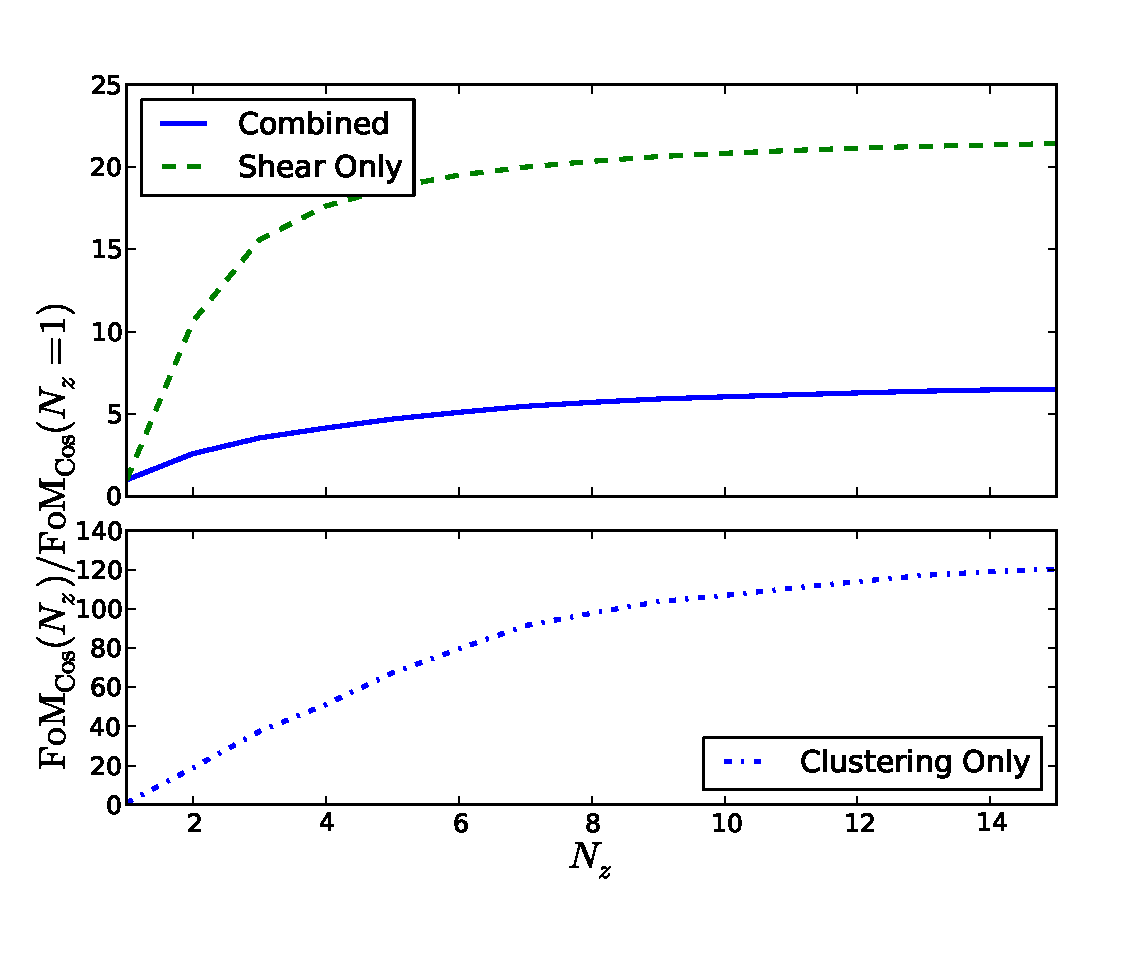
\includegraphics[width = 0.5\textwidth]{FoM_Nz.pdf}
\caption{Figure of merit (FoM$_{\rm Cos}$) as a function of number of redshift bins, for an S4 survey and for a shear only (green, dashed), clustering only (red dot-dashed) and combined (blue, solid) analysis.}\label{Fig:FoM_Nz}
\end{figure}

For the combined case, we see that the gains in information from further subdivision of the galaxy distribution are dominated by the gains in the shear analysis. Again, this is to be expected, comparing the figure of merit for an shear only and clustering only analysis, we see that there is much more information from the shear analysis, due to differences in the level of shot noise, as well as the fact that we are forced to cut much of the data in our magnification analysis to avoid probing the regime where the galaxy bias is expected to be non-linear.


\subsection{The effect of cross correlations in a photometric clustering analysis}\label{Sec:AutoClustering_v_Full}
Traditionally, spectroscopic clustering analyses which aim to constrain cosmological parameters consider only the auto-correlations of redshift bins, and ignore the clustering cross correlations between separated redshift bins where the magnification bias contribution to the overall power is larger. In this section, we question what gains can be made to a photometric clustering analysis when these cross correlations are also included, and whether there is a notable gain to constraints on cosmological parameters when  combined with a cosmic shear analysis.

Using the Fisher matrix formalism of Section \ref{Sec:FM_Clustering_Auto}, we present forecasts for our S4 survey, for two cases: For a clustering analysis which contains only the auto correlation power spectra, and for a clustering analysis which includes all redshift bin combinations.

Figure \ref{Fig:AutoClustering_v_Full} shows marginal constraints in the dark energy parameter ($\Omega_\lambda, w$) plane, for two different values for the slope of source number counts $\alpha$. The left column shows contours when $\alpha = 1$, the case when the clustering power spectrum contains no magnification bias contribution. In this case, any improvement to cosmological parameter constraints comes from the addition of the intrinsic clustering signal between separated redshift bins, which may be non-zero due to photometric redshift errors. On the right column, we present contours for $\alpha = 0.7$, the value measured from CFHTLenS data as described in Section \ref{Sec:CFHT}. In this case, there is a contribution to the clustering power spectrum from the inclusion of magnification bias effects. Top panels show contours for a clustering only analysis, and bottom panels show contours when the clustering analysis is combined with galaxy ellipticity measurements.

\begin{figure}
\centering
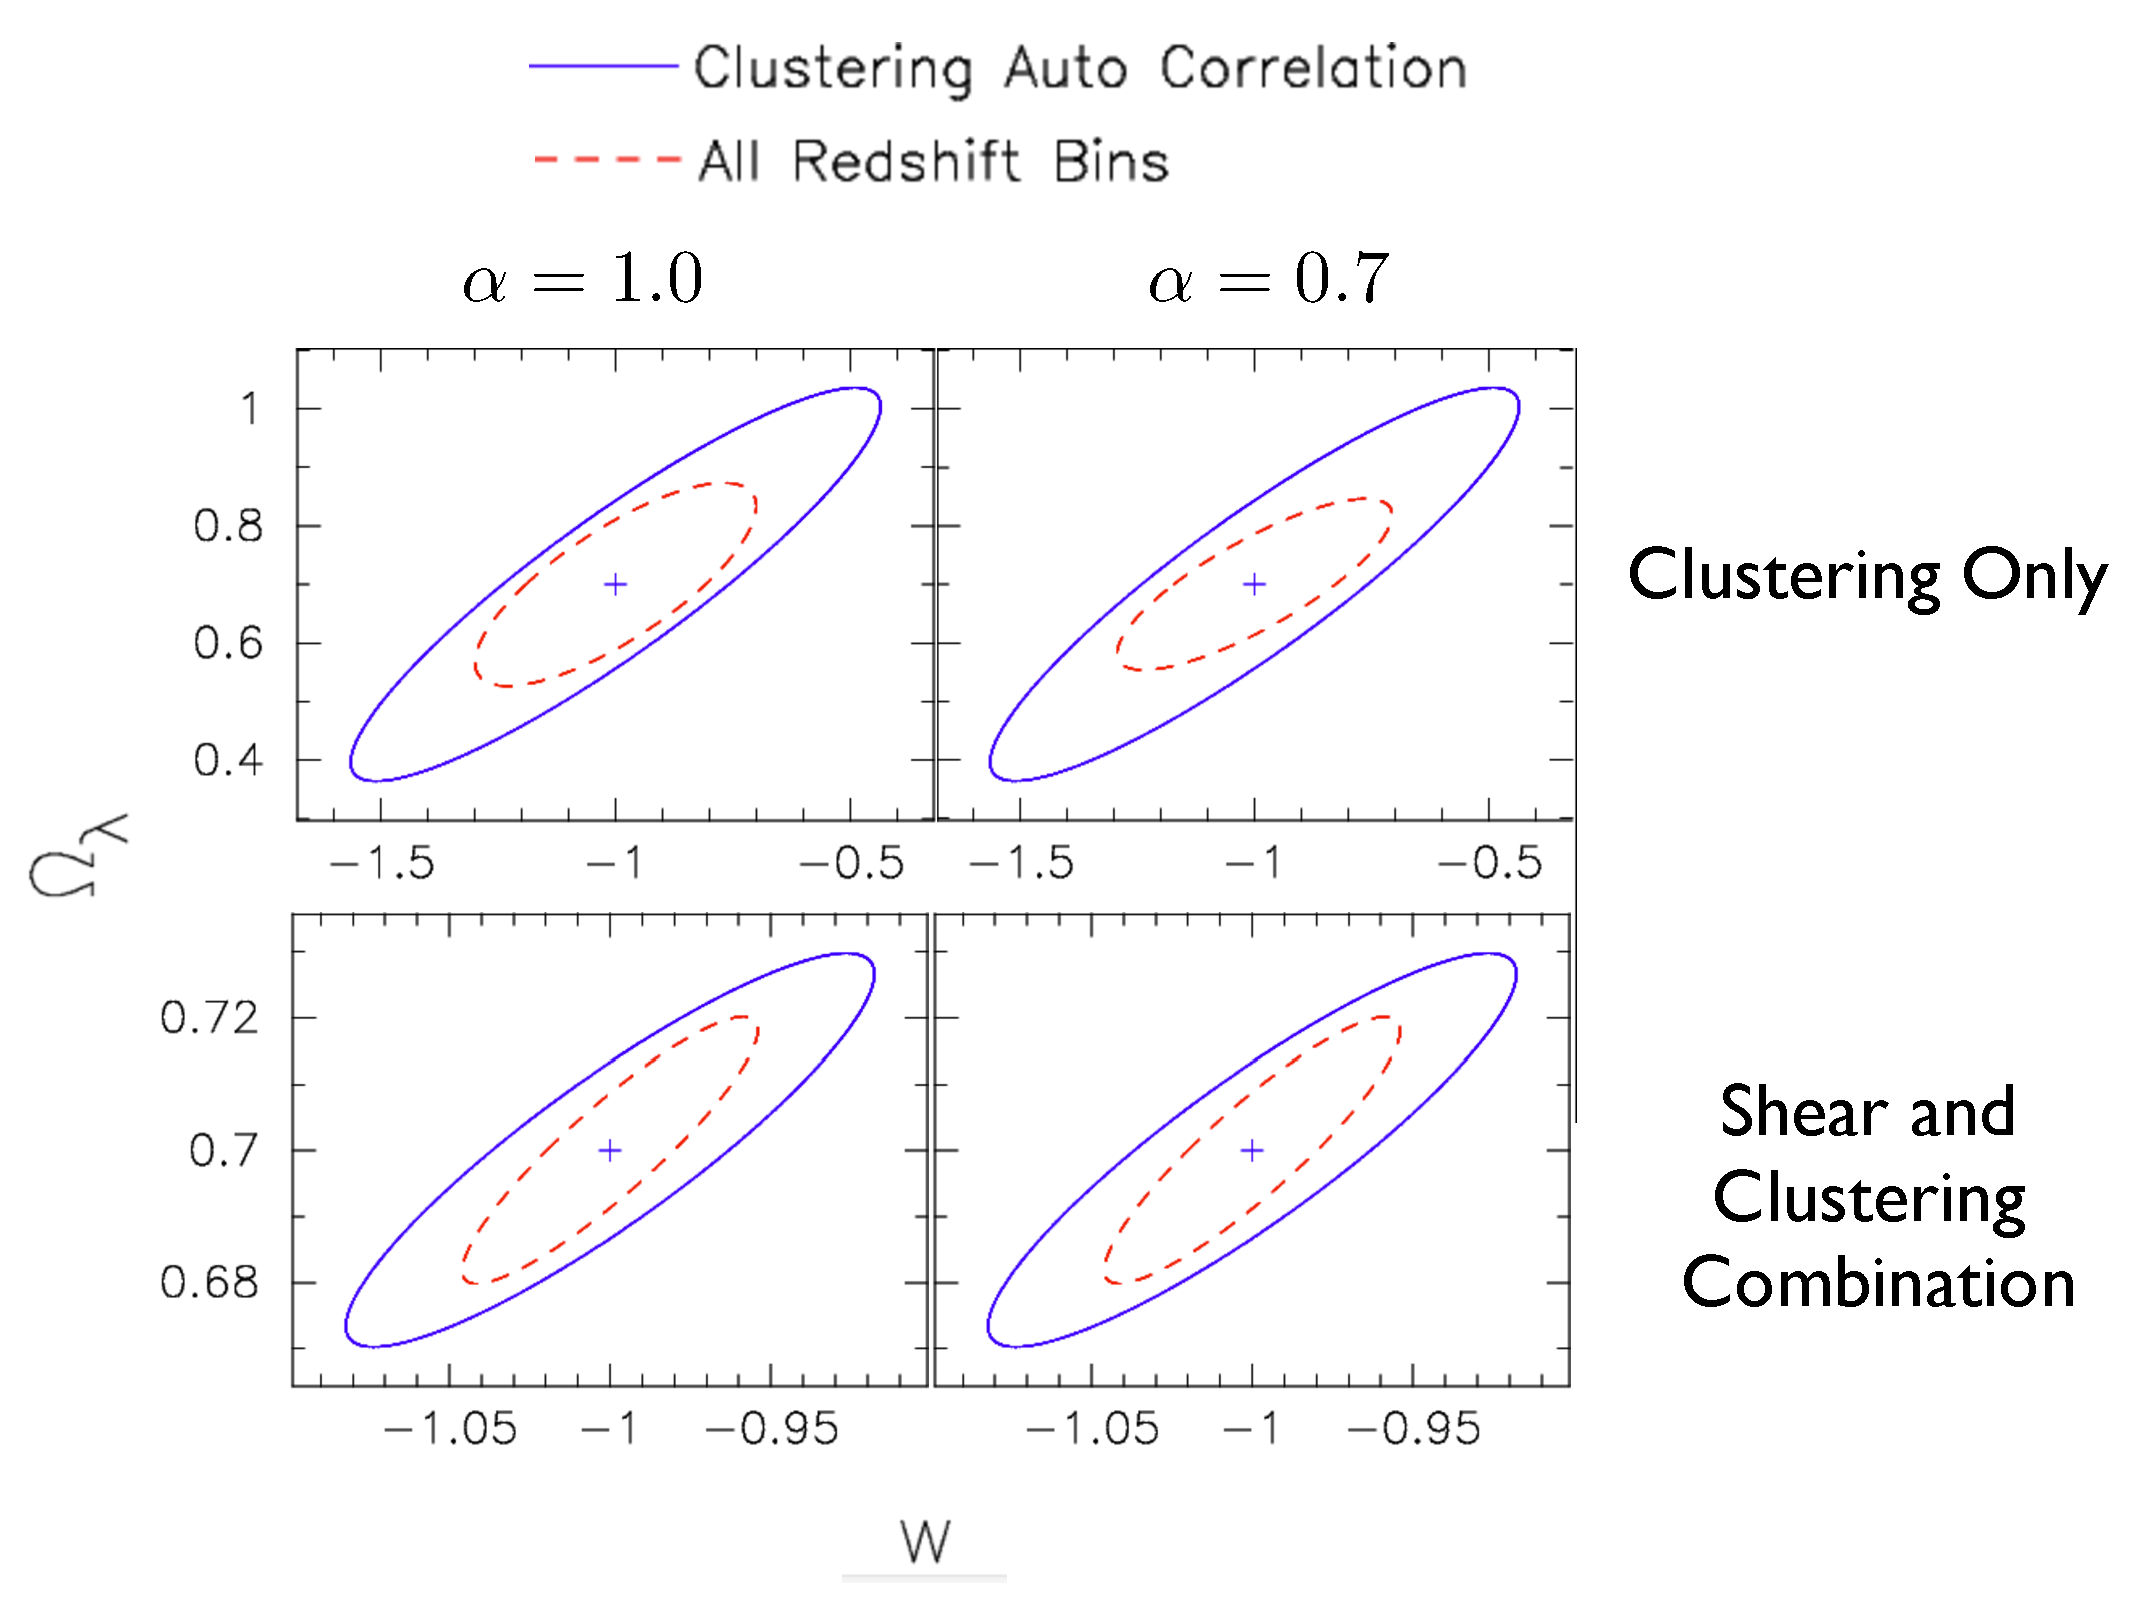
\includegraphics[width = 0.5\textwidth]{AutoClustering_v_Full.pdf}
\caption{Fisher Matrix forecast showing marginal constraints in  $w$, $\Omega_\lambda$  for an S4 survey, comparing measurements using only the auto power for the clustering signal (blue, solid), to measurements using all redshift bin combinations in the clustering analysis (red, dashed). The left column shows contours when $\alpha = 1$, the case when there are no measured correlations in the number density contrast due to magnification bias, and only correlations due to intrinsic clustering. The right column shows contours when $\alpha = 0.7$, as measured from CFHTLenS catalogues in Section \ref{Sec:CFHT}. Top panels show contours using clustering only, and bottom panels show contours when the clustering information is added to a cosmic shear analysis. All panels take unknown galaxy bias, and cut information from clustering on non-linear scales.}\label{Fig:AutoClustering_v_Full}
\end{figure}


From Figure \ref{Fig:AutoClustering_v_Full} we note that there is a significant improvement to parameter constraints when all combinations of redshift bins are included in a clustering analysis, showing a decrease by a factor of $\sim 2$ for statistical errors in $w$, and $\sim 1.6$ in $\Omega_\lambda$, and notably more when $\alpha \ne 1$ and there is a contribution from magnification bias. This improvement is still noticeable when the clustering analysis is combined with a shear analysis, and the addition of cross power spectra to the clustering give a decrease of $\sim 1.7$ and $\sim 1.5$ in statistical errors on $w$ and $\Omega_\lambda$ respectively. In contrast to the clustering only analysis, there is no noticeable difference in statistical errors when $\alpha \ne 1$ for the combined case, this agrees with the results detailed in Section \ref{Sec:Constraints_AlphaDependance}. We note that auto clustering does not significantly improve constraints form a shear analysis, and only improves errors on $\Omega_\lambda$ and $w_0$ by a factor of $\sim 10\%$, much less than the combination with clustering using all redshift bins.

We therefore conclude that there is significant gain in considering all redshift bin combinations in the clustering signal rather than the auto power only, even when combined with a cosmic shear analysis.

\subsection{Biases on cosmological parameters}

We finally turn our attention away from constraints on cosmological parameters to possible shifts in the deduced maximum likelihood point when fitting to data using only the intrinsic clustering power spectrum, and ignoring the contribution to the power spectrum from the magnification effect. To do this, we consider the linear shift in inferred parameters $(Q)$ due to a bias in fixed model parameters ($\psi$) using the formalism of \cite{Taylor:2007p1037}
\be\label{eqn:ParameterBias}
\bm{\delta Q}_i = -\sum_{k,j}[\mathbfss{F}^{QQ}]^{-1}_{ik}\mathbfss{F}^{Q\psi}_{kj}\bm{\delta \psi}_j
\ee
where $\mathbfss{F}^{QQ}$ is the Fisher matrix of measured  cosmological parameters using the only the galaxy clustering signal using auto-correlations in redshift bins set out in Section \ref{Sec:FM_Clustering_Auto},  and $\mathbfss{F}^{Q\psi}$ is a pseudo-Fisher matrix between inferred and fixed model parameters using the same formalism. Our measured parameters consist of the cosmological parameter set described in Section \ref{Sec:ParameterForecasts} including $N_z$ galaxy bias parameters (where $N_z$ is the number of redshift bins). Our set of assumed parameters consist of one $\alpha$ value per redshift bin, so that $\delta \psi^i = \alpha^i_{\rm true} -  1$, where we have noted that  setting $\alpha = 1$ sets the contribution to number density contrast fluctuations from magnification identically zero, thus equivalent to fitting only using the intrinsic clustering power spectrum. As previously, we choose $\alpha_{\rm true} = \ATrue$.

The results are shown in Table \ref{Table:ParameterBiasResults}. We find that whilst ignoring magnification can bias inferred parameter values, that in most cases the shift in parameter values is small compared to the statistical error on each parameter, except for $n_{\rm spec}$ and $\sigma_8$ for the S4 survey. We note that the absolute shift in inferred parameter value is reasonably robust to changes in the survey as we move from an S3 survey to an S4 survey, however there is an increase in the significance of these biases as the statistic errors are much improved in an S4 survey.

Whilst we have discarded all but the auto power spectra in this analysis, it should be noted that induced cosmological parameter biases are worse whenever cross-correlations between redshift bins are used in a clustering analysis. This may be expected as for increasingly separated redshift bins, the intrinsic clustering correlations become smaller and correlations induced due to magnification bias increase, as can be seen in Figure \ref{Fig:NumberPowerSpectra}, causing inferred cosmological parameters to be largely biased. 

As the parameter biases when including all redshift bins can be of the order of the parameter value itself, it is clear that the cosmic magnification effect must be taken into consideration when considering a clustering analysis that includes redshift bin cross-correlations. In Section \ref{Sec:AutoClustering_v_Full} we noted that there is a significant improvement in cosmological parameter constraints by using all redshift bins in the clustering analysis, however this comes at the expense of the increased importance of correctly modelling the effect of magnification bias to avoid large biases in inferred cosmological parameters.

\begin{table*}
\begin{minipage}{126mm}
\centering
\begin{tabular}[]{l | c | c | c | c }
\hline
& \multicolumn{2}{|c|}{S3 Ground}&\multicolumn{2}{c|}{S4 Space} \\
\hline

& Bias & \% & Bias & \%\\
\hline
$\Omega_M$  & 			$0.0046$& 			$1.70$ & 	$0.0042$ & 			$5.54$\\
$\Omega_{\rm Baryon}$  &	$-0.70\times10^{-3}$& 	$-1.44$ & 	$-0.60\times10^{-3}$& 	$-4.33$\\
$\Omega_{\lambda}$  & 		$0.02$& 				$1.52$ & 	$0.027$& 				$8.00$\\
$w_o$  & 					$0.033$& 				$1.51$ & 	$0.046$& 				$8.11$\\
$h$ & 					$0.005$ & 			$0.63$ & 	$0.014$& 				$6.27$\\
$n_{\rm spec}$ & 			$-0.021$& 			$-8.90$ & 	$-0.027$& 			$-43.1$\\
$\sigma_8$  & 				$0.0081$& 			$6.82$ & 	$0.0095$& 			$28.3$\\
\hline
\end{tabular}
\caption{Biases on cosmological parameters from incorrectly fitting to clustering data using only the intrinsic clustering power spectrum. Results are shown for the case where parameter constraints come from number density auto-correlations in redshift bins for survey types defined in Section \ref{Sec:SurveyModelling}.  For each survey type, the absolute bias is shown with the percentage of the $1\sigma$ statistical error of each parameter.}\label{Table:ParameterBiasResults}
\end{minipage}
\end{table*}

\section{Conclusions}

In this paper we have forecast statistical errors on cosmological parameters from a cosmic shear analysis, and two types of photometric clustering analysis including magnification bias effects: one which contains information only from correlating all redshift bins with themselves (auto), and one where all redshift bin combinations are included, in the presence of contamination due to photometric redshift errors. We considered the gain from combining either clustering analysis with a shear analysis, to address recent suggestions that a combination of both can give significant gains in cosmological parameter constraints. %as suggested by....

To limit the impact of galaxy bias on non-linear scales, which is poorly understood, we applied cuts on clustering information on $\ell$-modes above which the r.m.s matter density fluctuations are larger than a given value. We found that by relaxing these cuts, constraints from a clustering analysis, as well as the combination of clustering with shear, improved significantly, suggesting that galaxy clustering will be a much more powerful tool in probing cosmology if non-linear clustering is better understood. We modelled the redshift dependance of the galaxy bias by applying a nuisance parameter for each redshift bin, each of which must be constrained by the data simultaneously. We found that some of the gain in constraining power by combining clustering information with shear was lost when the galaxy bias was unknown, suggesting that the results presented in \cite{VanWaerbeke:2010p8} would be too optimistic.

We investigated the sensitivity of the statistical errors on cosmological parameters to the magnification bias effect and found that when we consider clustering with all redshift bins, that there can be significant improvement to constraints when the clustering signal contains contribution from magnification bias. However, when combined with a cosmic shear analysis, any improvement to constraints due to magnification bias is weak, as the constraints on cosmological parameters from clustering are significantly smaller than those from shear, so any gain in constraints from a combination of both comes from degeneracy breaking.

We studied how statistical errors on cosmological parameters could be improved in a clustering analysis when all redshift bin combinations were included in the analysis, over the more traditional approach of using only the auto correlations in number density contrast within one redshift bin. We find that there is significant improvement in constraints from adding this extra information, with improvement by a factor of $\sim 1.5$ in statistical errors on dark energy parameters.

Finally, we questioned by how much would inferred parameter values be biased if the magnification bias effect was incorrectly ignored in a clustering analysis. We find that when the clustering analysis contains only the auto correlations, that biases are small compared to statistical errors on parameters, however we note that for our Stage IV space-based survey (with larger survey area and effective number density of galaxies), these biases are more significant due to the improved statistical errors, reaching $\sim 40\%$ for $n_{\rm spec}$ and $\sim 30\%$ for $\sigma_8$. We also found that when clustering data across all redshift bins was used, inferred parameters can be biased to the same order of magnitude as the parameter value themselves, and that these biases were much larger than the statistical error on each parameter, often by more than an order of magnitude. 

We therefore conclude that whilst adding clustering information to galaxy ellipticity measurements can significantly decrease statistical errors on cosmological parameters, most of this information gain comes from degeneracy breaking and is as such weakly dependent on the magnification bias contribution when the intrinsic clustering power is also included, as the statistical errors in a clustering analysis are much larger than a shear analysis when galaxy bias is unknown. As there is significant improvement to the statistical errors when all redshift bin combinations are used in a clustering analysis, even when combined with a shear analysis, we suggest that photometric clustering analyses should use all redshift bin information in inferring cosmological parameters, at the expense of increased complexity due to the increased necessity to accurately measure and model magnification bias to avoid biasing inferred cosmological parameters.

Similarly, we expect that the largest gains in combining number density contrast measurements with cosmic shear would come from using all available information across all redshift bins. As magnification bias measurements often only take widely separated bins to make the intrinsic clustering contribution sub dominant to the largest magnification bias contribution, we expect that the loss of information from not considering the full sample and also modelling the intrinsic clustering would increase statistical errors on cosmological parameters. %FUTURE WORK?

As much of the extra information gained from the addition of clustering data to ellipticity measurements is lost when the galaxy bias must also be constrained with the data, and when clustering information is cut on non-linear scales, we suggest that the largest improvements will be made with better knowledge of galaxy bias and non-linear clustering. 

{\bf We note that as well as the improvement in statistical errors that comes from adding clustering measurements to cosmic shear, number density information gives an important consistency check on inferred cosmological parameters, allowing independent verification of inferred parameter values using either number density contrast correlations, or galaxy-galaxy lensing, and an important consistency check. As the information required for a photometric clustering analysis is already taken as part of a shear survey, this information is obtained for free.}

%Alpha dependance

%Adding all redshift bin information

%Parameter Biases

%Conclusion - we suggest that all redshift bins must be considered, but that the importance of accurately measuring and modelling the mag bias effect increases....

\section*{Acknowledgments}

Catherine Heymans acknowledges support from the European Research Council under the EC FP7 grant number 240185.

\bibliographystyle{mn2e}
\bibliography{Papers_BIBTEX}

\appendix

\section[]{The Galaxy Bias Prior - Normalising the Likelihood}\label{App:NormalisingGBP}

We define the covariance matrix for the prior on $N_z$ linear galaxy bias parameters as in Equation (\ref{Eqn:BiasPriorCov}). The covariance matrix then takes the form $\mathbfss{C} = \sigma_r^2 \mathbfss{R}$, where $\mathbfss{R}$ is the matrix of correlation parameters ($\nu$) in Toeplitz form. Assuming the full likelihood for the bias parameters is Gaussina, it then follows:
\be
\frac{p(\bar{b})}{p(\bar{0})}  =  e^{-\frac{1}{2}\chi^2}
\ee
 where $\bar{b}$ labels the set of galaxy bias nuisance parameters, we have renormalised to the likelihood when $\bar{b} = \bar{0}$ to remove any prefactors, and
 \bea
 \chi^2 & = &\bm{b}\mathbfss{C}^{-1}\bm{b}^T\nonumber\\
 &=& \sum_{ij} ^{N_z} b^2 (\mathbfss{C}^{-1})_{ij}
 \eea
 along the line $b_1 = b_2 = \cdot\cdot\cdot = b_{N_z} = b$. From the definition of the covariance matrix in Equation (\ref{Eqn:BiasPriorCov}) It follows that
  \begin{eqnarray}
   \chi^2 &=& \frac{b^2}{\sigma_\nu^2}\sum_{ij}^n (\mathbfss{R}^{-1})_{ij} = \frac{b^2}{\sigma_\nu^2}\sum_{ij}^{N_z} \left[\frac{\mathbfss{Adj}(\mathbfss{R})}{{\rm det}(\mathbfss{R})}\right]_{ij} \nonumber\\ &=& \frac{b^2}{\sigma_\nu^2 {\rm det}(\mathbfss{R})}\sum_{ij}^{N_z} [\mathbfss{Co}(\mathbfss{R})^{\rm T}]_{ij}\nonumber\\
 &=&  \frac{b^2}{\sigma_\nu^2 {\rm det}(\mathbfss{R})}\sum_{ij}^{N_z} [ \mathbfss{Co}(\mathbfss{R})]_{ij} \label{eqn:nChi}
 \end{eqnarray}
 where $\mathbfss{Adj}(R)$ denotes the adjoint matrix of $\mathbfss{R}$, $\mathbfss{Co}(\mathbfss{R})$ the matrix of cofactors, defined as $ {\rm Co(\mathbfss{R})}_{ij} = (-1)^{i+j}{\rm M}_{ij}$, $\mathbfss{M}$ the minor matrix of determinants, and we have used the symmetry of $R$ to note that $\mathbfss{Co}(\mathbfss{R})^{\rm T} = \mathbfss{Co}(\mathbfss{R})$. 
  
By the symmetry of $\mathbfss{R}$, and the definition of the minor matrix of determinants, the matrix of cofactors  $\mathbfss{Co}(\mathbfss{R})$ satisfies %by mathematica algebra?
\be
\mathbfss{Co}(\mathbfss{R}) = \begin{pmatrix} x_1 & x_2 & 0 & 0 & \cdots & 0 \\  x_2 & x_3 & x_2 & 0 & \cdots & 0 \\ 0 & x_2 & x_3 & x_2 & \cdots & 0 \\ \vdots &  & \ddots &  &  & \vdots \\  0 & \cdots & 0 & 0 & x_2 & x_1 \end{pmatrix}
\ee
so that
 \be\label{eqn:SumCo}
 \sum_{ij}^n \mathbfss{ Co}(\mathbfss{R})_{ij} = 2x_1 + 2(N_z-1)x_2 + (N_z-2)x_3.
 \ee
 and ${\rm det}(\mathbfss{R}) = (1-\nu^2)^{N_z-1}$.  Variable $x_1$ is the determinant of the $N_z-1$ case of the matrix $\mathbfss{R}$, which I denote as ${\rm det}(\mathbfss{R}^{(N_z-1)})$. The remaining factors can be calculated by noting that
 \be
 \sum_{j}^{N_z} \mathbfss{R}_{ij} \mathbfss{Co}(\mathbfss{R})_{ij} = {\rm det}(\mathbfss{R})
 \ee
 so that 
 \begin{eqnarray}
x_2 &=& \frac{1}{r}[{\rm det}(\mathbfss{R}^{(N_z)}) - {\rm det}(\mathbfss{R}^{(N_z-1)})] \\
x_3 &=& 2{\rm det}(\mathbfss{R}^{(N_z-1)}) - {\rm det}(\mathbfss{R}^{(N_z)}).
\end{eqnarray}

Using Equations (\ref{eqn:SumCo}) and (\ref{eqn:nChi}), we find that 
\be
 \chi^2 = \frac{b^2}{\sigma_\nu^2}\left[\frac{N_z-(N_z-2)\nu}{1+\nu}\right].
 \ee
It is clear then that if we keep $\sigma_\nu$ constant with $\nu$, $\chi^2$ at a given point along the $b_1 = b_2 = \cdot\cdot\cdot = b_{N_z} = b$ line will vary with $\nu$ causing a change in the volume of galaxy bias parameter space probed by $1-\sigma$ contours to also vary with the correlation strength. We therefore normalise $\chi^2$ along $b_i = b$ by choosing $\sigma_\nu$ such that $\chi^2_\nu = \chi^2_{\nu=0}$ for all values of $\nu$. Noting that by Pythagoras' theorem $b = \sigma_0/\sqrt{N_z}$ and requiring that $\sigma_\nu(\nu=0) = \sigma_0$, we find that
 \be
 \sigma_\nu = \sigma_0\left[\frac{N_z-(N_z-2)\nu}{N_z(1+\nu)}\right]^{\frac{1}{2}}
 \ee
  as stated in Equation (\ref{eqn:BP_sigr_sig0}).

\bsp

\label{lastpage}

\end{document}
